\documentclass[letterpaper,landscape]{slides}
%\documentclass[letterpaper,portrait]{slides}
\usepackage{boxedminipage}

%\input /u/rhl/TeX/pdf.tex
\input pdf.tex

\newif\ifTalk\Talktrue		% We generating a talk, not printing
%\Talkfalse			% no; we're really printing

%\pagestyle{empty}
\setlength{\topmargin}{-1in}
\setlength{\textheight}{7.5in}
\setlength{\textwidth}{9in}
\setlength{\oddsidemargin}{0pt}
\setlength{\oddsidemargin}{0pt}

%\onlyslides{1-3,4,10-9999}
%\onlyslides{26-9999}

\begin{document}

\newcommand{\XXX}[1]{\textbf{XXX} #1}
\newcommand{\colour}[1]{\color{#1}}

\def\eq#1{\begin{equation} \color{blue} #1 \end{equation}}

\def\b#1{{\bf  #1}}
\def\p{\partial}
\def\th{^{th}}
\def\msun{{\rm\,M_\odot}}
\def\bnabla{{\bf\nabla}}
\def\dint{\int\!\!\!\int}
\def\d{{\rm d}}
\def\i{{\rm i}}
\def\ddt#1{{\rm{d} #1\over {\rm dt}}}
\def\ddtS#1{{\rm{d^2} #1\over {\rm dt^2}}}
%\lta and \gta produce > and < signs with twiddle underneath
\def\spose#1{\hbox to 0pt{#1\hss}}
\def\lta{\mathrel{\spose{\lower 3pt\hbox{$\mathchar"218$}}
     \raise 2.0pt\hbox{$\mathchar"13C$}}}
\def\gta{\mathrel{\spose{\lower 3pt\hbox{$\mathchar"218$}}
     \raise 2.0pt\hbox{$\mathchar"13E$}}}
\def\mspace{\hbox{\quad}}

\def\deffn#1{{\bf#1}}\def\eqs#1{equations \rf#1}


\newcount\itemCnt\itemCnt=0
\newcommand{\nitem}{%
  \global\advance\itemCnt by 1
  ~\vskip0cm\the\itemCnt.\qquad}

\definecolor{orange}{rgb}{1.0, 0.5, 0.0}
\definecolor{purple}{cmyk}{0.4, 0.8, 0.3, 0.0}


%%%%%%%%%%%%%%%%%%%%%%%%%%%%%%%%%%%
\newcommand{\onepic}[6]{%
\begin{slide}
     \begin{center}
        \begin{minipage}{#1in}
            {\large \color{blue} #6}
            \phantom{x} \vskip #2in
            \phantom{x} \hskip #3in
            {\scalebox{#4}{\includegraphics{#5}}}   
        \end{minipage}
     \end{center}
    \vfill
\end{slide}
}


%%%%%%%%%%%%%%%%%%%%%%%%%%%%%%%%%%%
\newcommand{\picslide}[7]{%
  \begin{slide}
     \begin{center}
        \begin{minipage}{#5in}
            \hskip #6in
            \hskip -1in
            {\scalebox{#4}{\includegraphics{#1.#2}}}
            \vskip #7in~
            {\large \color{blue} #3}
        \end{minipage}
     \end{center}
     \vfill
  \end{slide}
}
%%%%%%%%%%%%%%%%%%%%%%%%%%%%%%%%%%%
 

%------------------------------------------------------------------------------
%------------------------------------------------------------------------------

\begin{slide}

\phantom{x}
\vskip -2in
\begin{center}
\bfseries
{\large {\color{blue} Astr 511: Galaxies as galaxies}}
\end{center}

{\centerline {{\color{blue} 
Winter Quarter 2017, University of Washington}}}
{\centerline {{\color{blue} 
Mario Juri\'{c} \& \v{Z}eljko Ivezi\'{c} }}}

\vskip 1.6in

{\centerline {\huge {\color{red}      Lecture 4:             }}}
\vskip 0.2in 
{\centerline {\Large {\color{blue}  Luminosity and mass functions  }}}

\vfill
\end{slide}
%------------------------------------------------------------------------------


%------------------------------------------------------------------------------
\begin{slide}
\begin{center}
\bfseries
{\large {\color{red} Outline}}
\end{center}
\vskip 0.2in
\hrule

\begin{itemize}
\item Galaxies as seen by SDSS
\item Luminosity function: basic concepts
\item Methods for estimating LF from data
\item Stellar mass function in the Milky Way 
\end{itemize}


\vfill
\end{slide}
%------------------------------------------------------------------------------








%------------------------------------------------------------------------------

\begin{slide}

\begin{center}
\bfseries
{\color{red} \large Galaxies in SDSS-I}
\end{center}
 \vskip 0.2in
\hrule

\begin{itemize}
\item
{\color{red}Imaging Survey}
   \begin{itemize}
   \item 10,000 deg$^2$ (1/4 of the full sky)
   \item 5 bands (ugriz: UV-IR), 0.02 mag photometric accuracy
   \item $<0.1$ arcsec astrometric accuracy
   \item 100,000,000 stars and 100,000,000 galaxies
   \end{itemize}

\item
{\color{red}Spectroscopic Survey}
   \begin{itemize}
   \item 1,000,000 galaxies
   \item 100,000 quasars
   \item 100,000 stars
   \end{itemize}

\end{itemize}
\end{slide}
 

%------------------------------------------------------------------------------


%------------------------------------------------------------------------------

\begin{slide}
\begin{center}
{\large \color{red} SDSS Spectroscopic Galaxy Survey }
\end{center}

\begin{itemize}
\item
{\color{blue} Two samples:} 
\begin{enumerate} 
\item the ``main'' galaxy sample ($r_{Pet}<17.77$): $\sim$1 million spectra
\item luminous red galaxy sample (LRG, cut in color-magnitude space): $\sim$100,000 spectra
\end{enumerate}  
\item
Distance estimate allows the determination of luminosity function (Blanton
et al. 2001)
\item Spectra are correlated with morphology (and colors)
\end{itemize}  

\vfill
\end{slide}
%------------------------------------------------------------------------------


%------------------------------------------------------------------------------
\begin{slide}
\begin{center}
\scalebox{0.5}{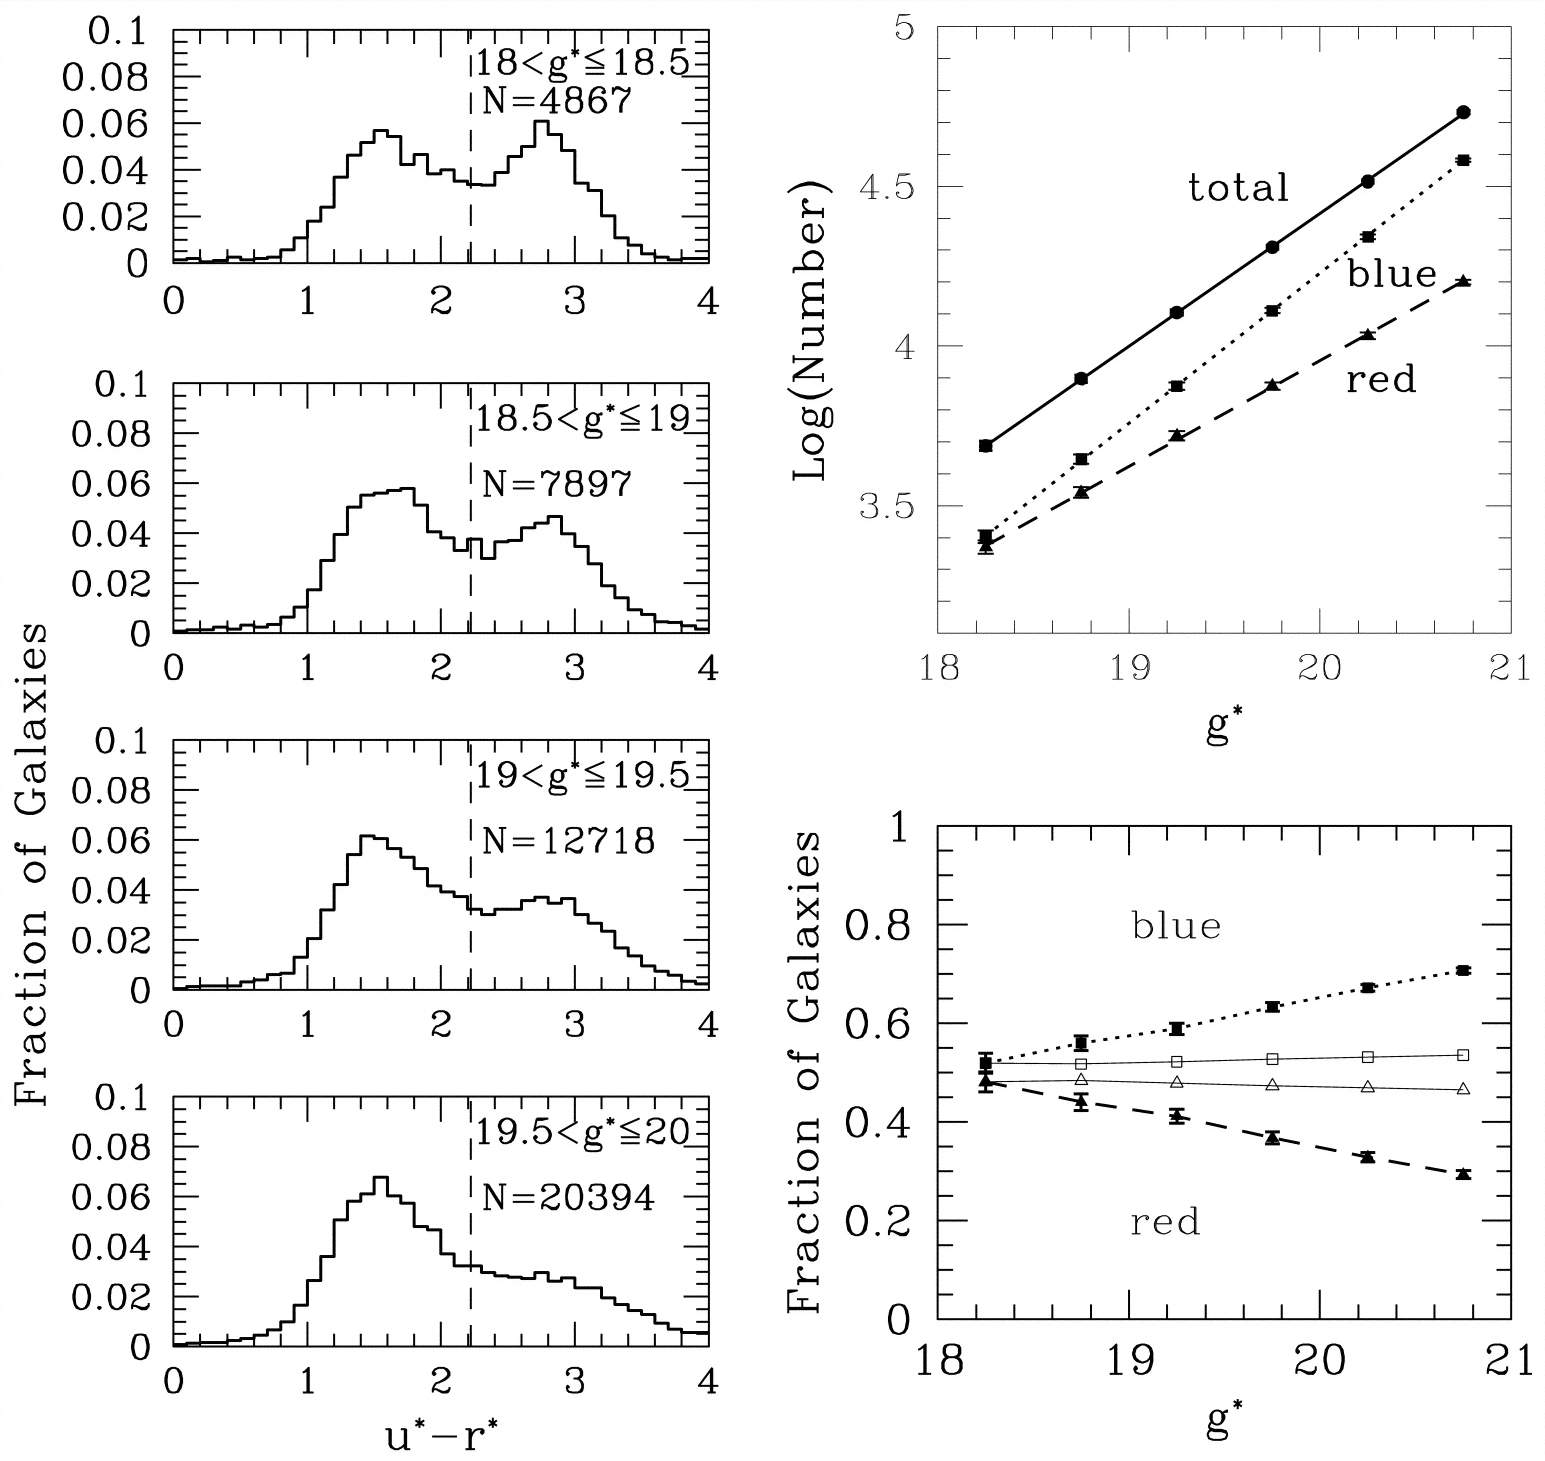
\includegraphics{figures/Strateva_fg2.jpg}}
\end{center}
Strateva et al. (2001, AJ 122, 1861): {\color{red} bimodal $u-r$ color distribution} ($u-r$ is similar to $U-V$)
\vfill
\end{slide}
%------------------------------------------------------------------------------

\begin{slide}
\begin{center}
\scalebox{0.6}{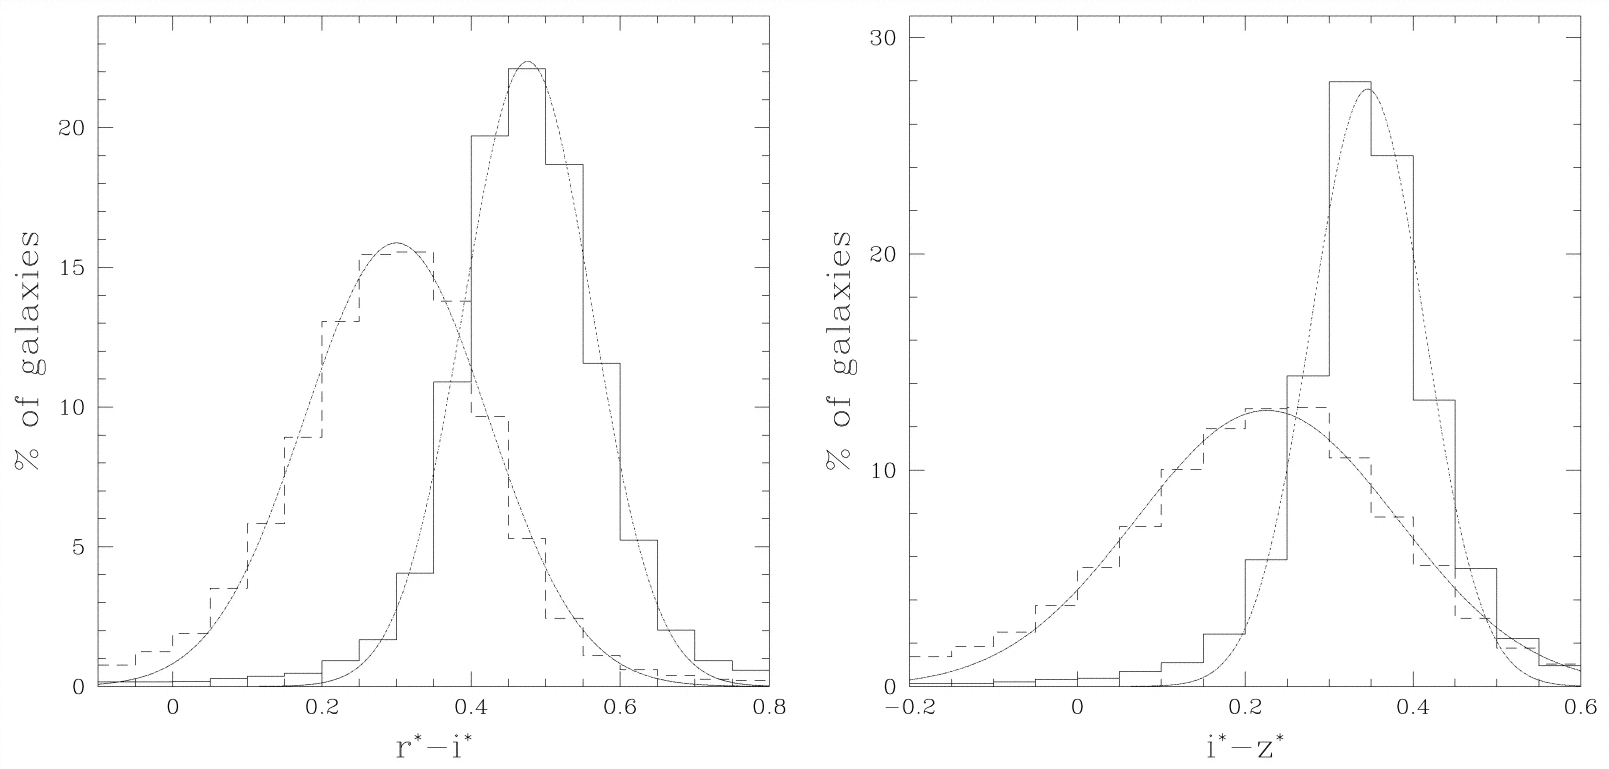
\includegraphics{figures/Strateva_fg3.jpg}}
\end{center}
{\color{blue} The broad band SEDs of galaxies are nearly one-dimensional family.}

{\color{red} ``Everything is correlated with everything'' (Blanton et al. 2003)}
\vfill
\end{slide}
%------------------------------------------------------------------------------



 
%------------------------------------------------------------------------------
% TWO-SIDED PAGE 
\begin{slide}

\hbox to \hsize{
\begin{minipage}[t]{13cm}
\begin{center}
\vskip 0.1in
\scalebox{0.65}{\hskip -1.6in 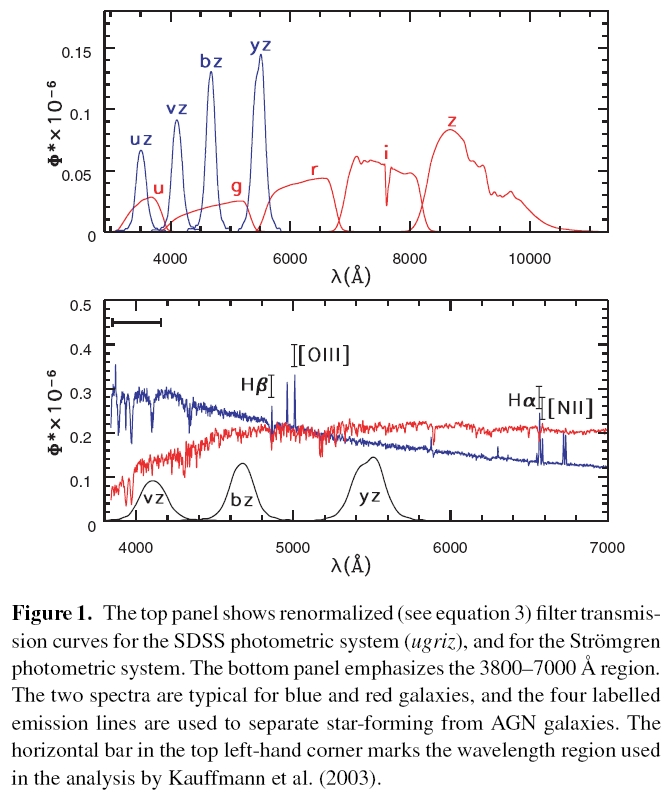
\includegraphics{figures/smolcic_fig1.jpg}}

\end{center}
\end{minipage}

\begin{minipage}[t]{11.5cm}
\vskip -1in
\begin{itemize}
\item
{\large \color{red} Star formation vs AGN}
\item
{\color{blue} It is not easy to distinguish galaxies with active star formation 
from those that harbour an AGN} (active galactic nuclues; a.k.a. black hole with 
an accretion disk)
\item We can use the emission line strength to separate them: 
$H_\alpha$, $H_\beta$, $[NII]$, $[OIII]$
\item {\color{blue} Physical origin: AGN have power-law spectra, so they have 
more UV photons than even the hottest stars;} as a result, for
a given $[OIII]/H_\beta$ ratio, AGNs have larger $[NII]/H_\alpha$ 
ratio than star-forming galaxies
\end{itemize}  

\end{minipage}}
\vfill 
\end{slide}
%------------------------------------------------------------------------------


%------------------------------------------------------------------------------
% TWO-SIDED PAGE 
\begin{slide}

\hbox to \hsize{
\begin{minipage}[t]{10cm}
\begin{center}
\vskip -0.7in
\scalebox{0.85}{\hskip -1.8in 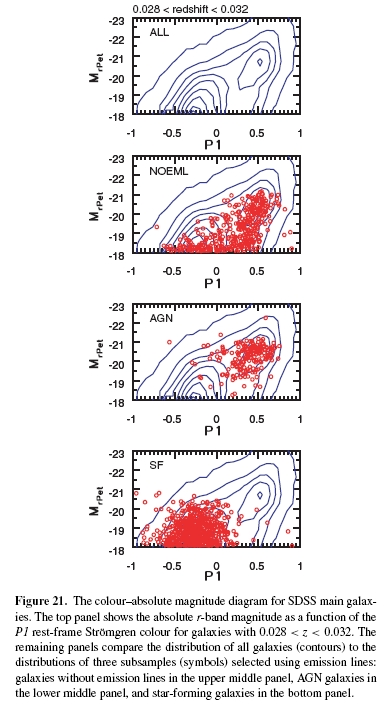
\includegraphics{figures/smolcic_fig21.jpg}}

\end{center}
\end{minipage}

\begin{minipage}[t]{14cm}
\vskip -1in
\begin{itemize}
\item
{\large \color{red} Correlations of Galaxy Parameters}
\item
{\color{blue} Many physical parameters are correlated with each other}; for example,
the luminosity, concentration of the light profile, and spectral line 
strengths are correlated with colors
\item
In the color-color space, galaxies form a very thin locus: {\color{blue} the SEDs of
galaxies are nearly one-dimensional family} (at the level of $\sim$0.02 mag)
\item Next page: SDSS sample from Blanton et al. (2003); the quantities
are $u-g$, $g-r$, $r-i$ and $i-z$ colors, surface brightness, Sersic index,
and absolute magnitude in the $r$ band; the grayscale plots show galaxy 
distribution in 2D diagrams, together with distributions of each individual 
quantity (histograms).
\end{itemize}  

\end{minipage}}
\vfill 
\end{slide}
%------------------------------------------------------------------------------



\begin{slide}
\begin{center}
\scalebox{0.37}{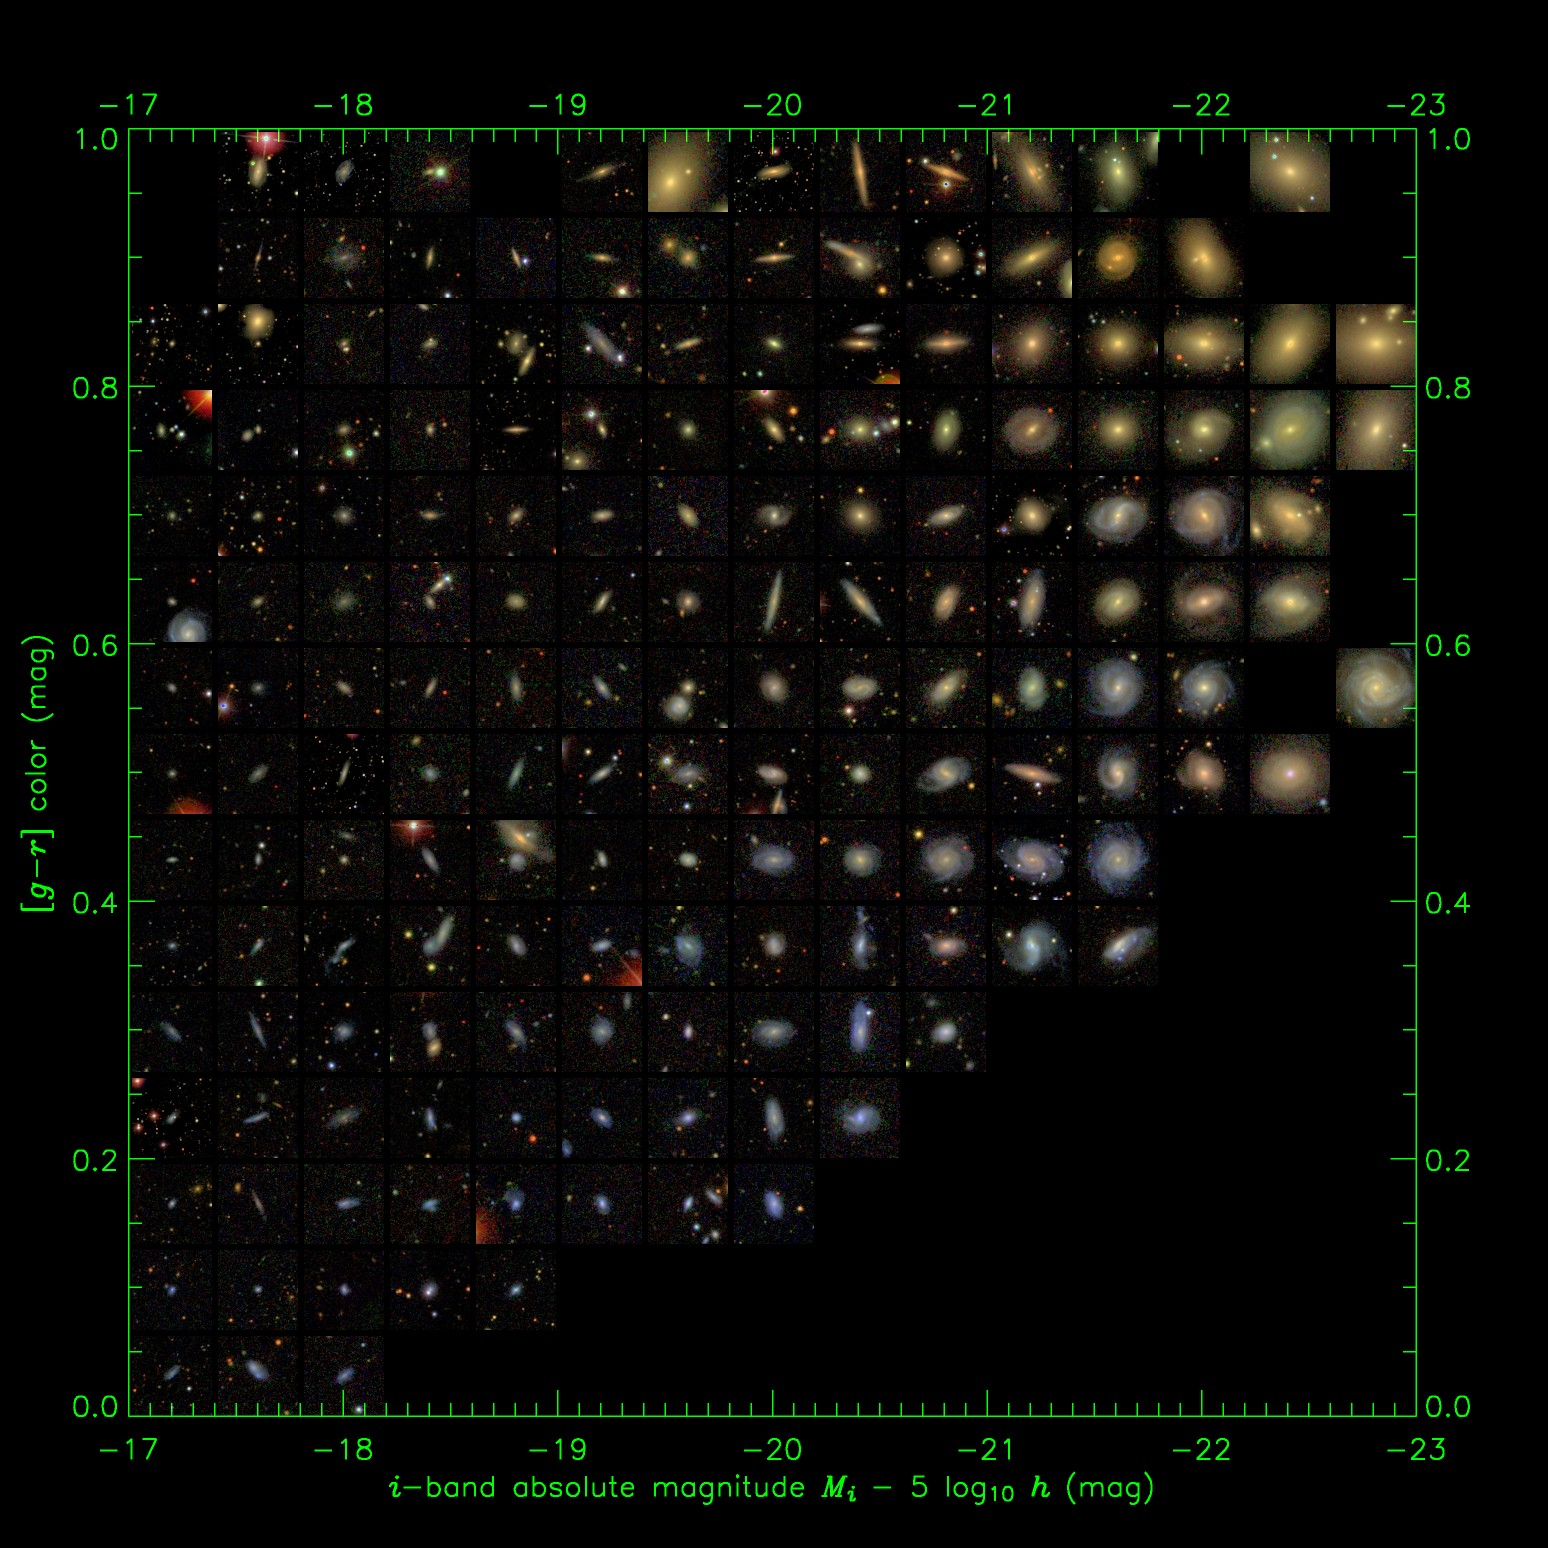
\includegraphics{figures/BHcolor-mag1.jpg}}
\end{center}
\vfill
\end{slide}
%------------------------------------------------------------------------------



\begin{slide}
\begin{center}
\scalebox{0.6}{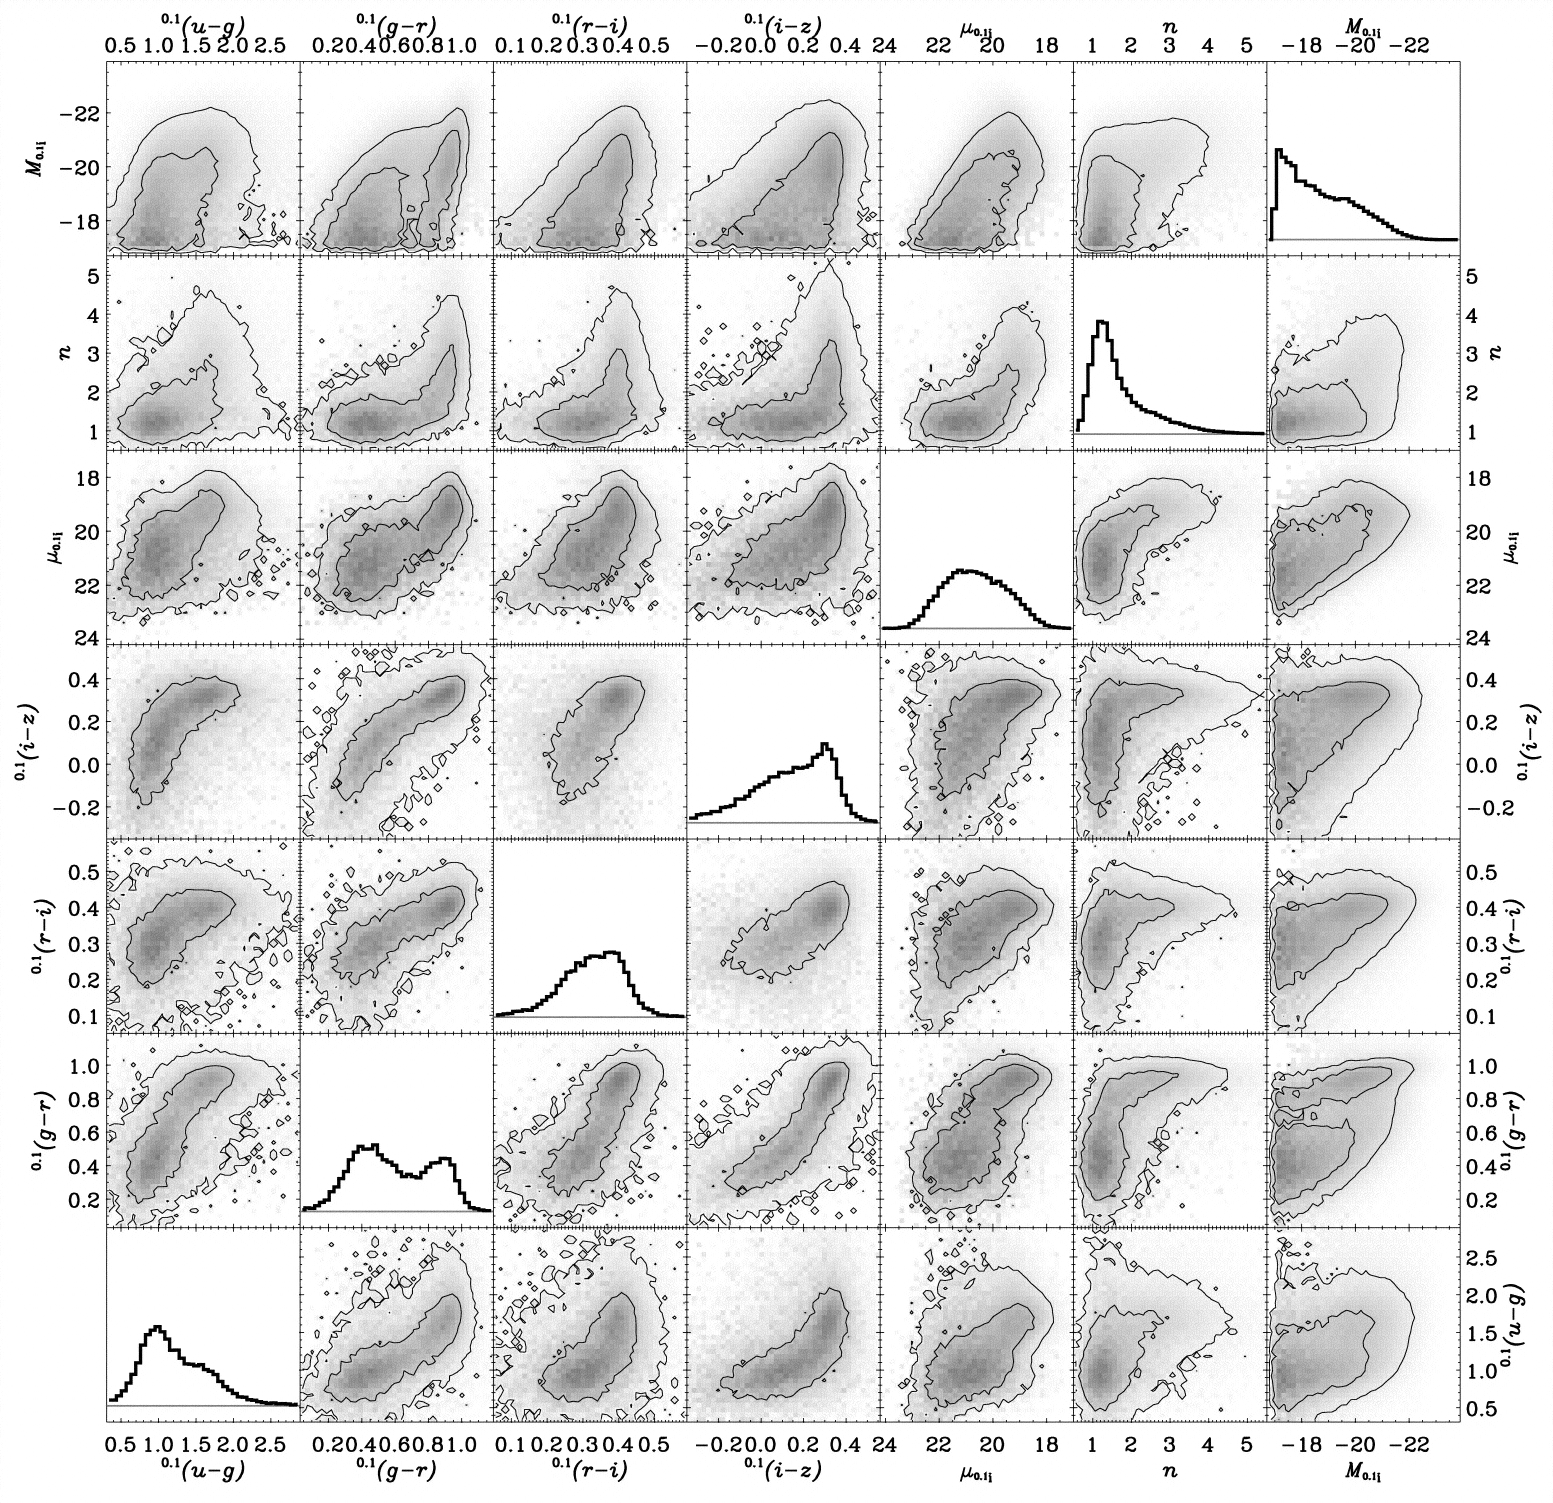
\includegraphics{figures/Blanton_7D.jpg}}
\end{center}
\vfill
\end{slide}
%------------------------------------------------------------------------------




%%%

\begin{slide}
\begin{center}
\scalebox{0.6}{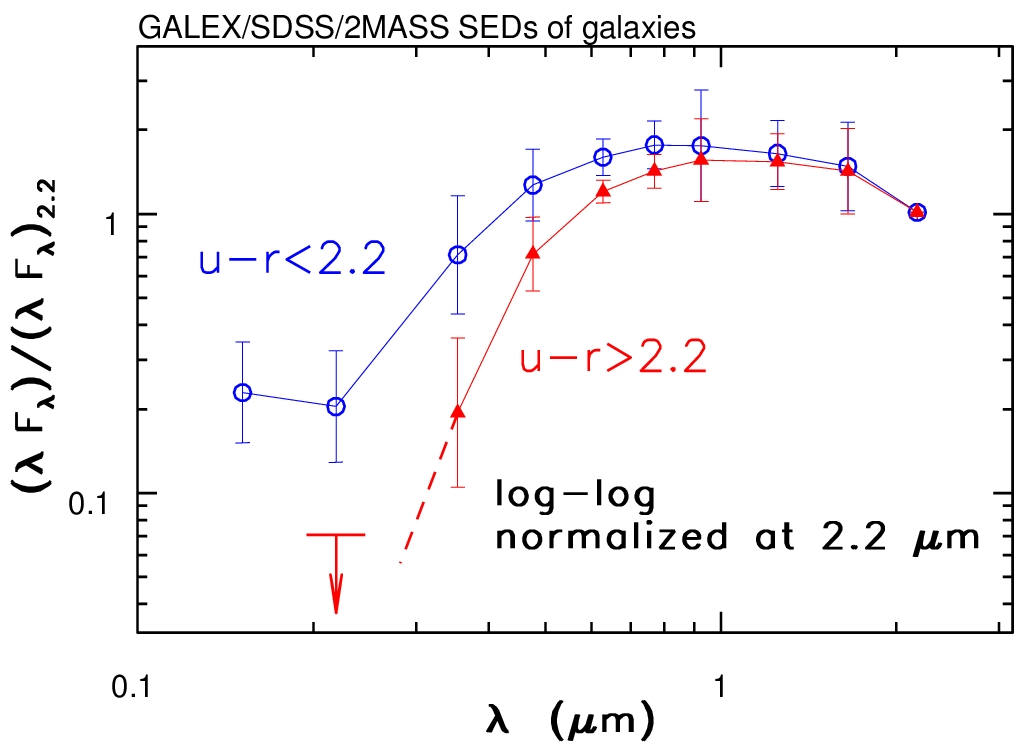
\includegraphics{figures/10bandSEDgalaxies.jpg}}
\end{center}
\vfill
\end{slide}
%------------------------------------------------------------------------------



%------------------------------------------------------------------------------
% TWO-SIDED PAGE 
\begin{slide}

\hbox to \hsize{
\begin{minipage}[t]{13cm}
\begin{center}
\vskip 0.1in
\scalebox{0.45}{\hskip -1.8in 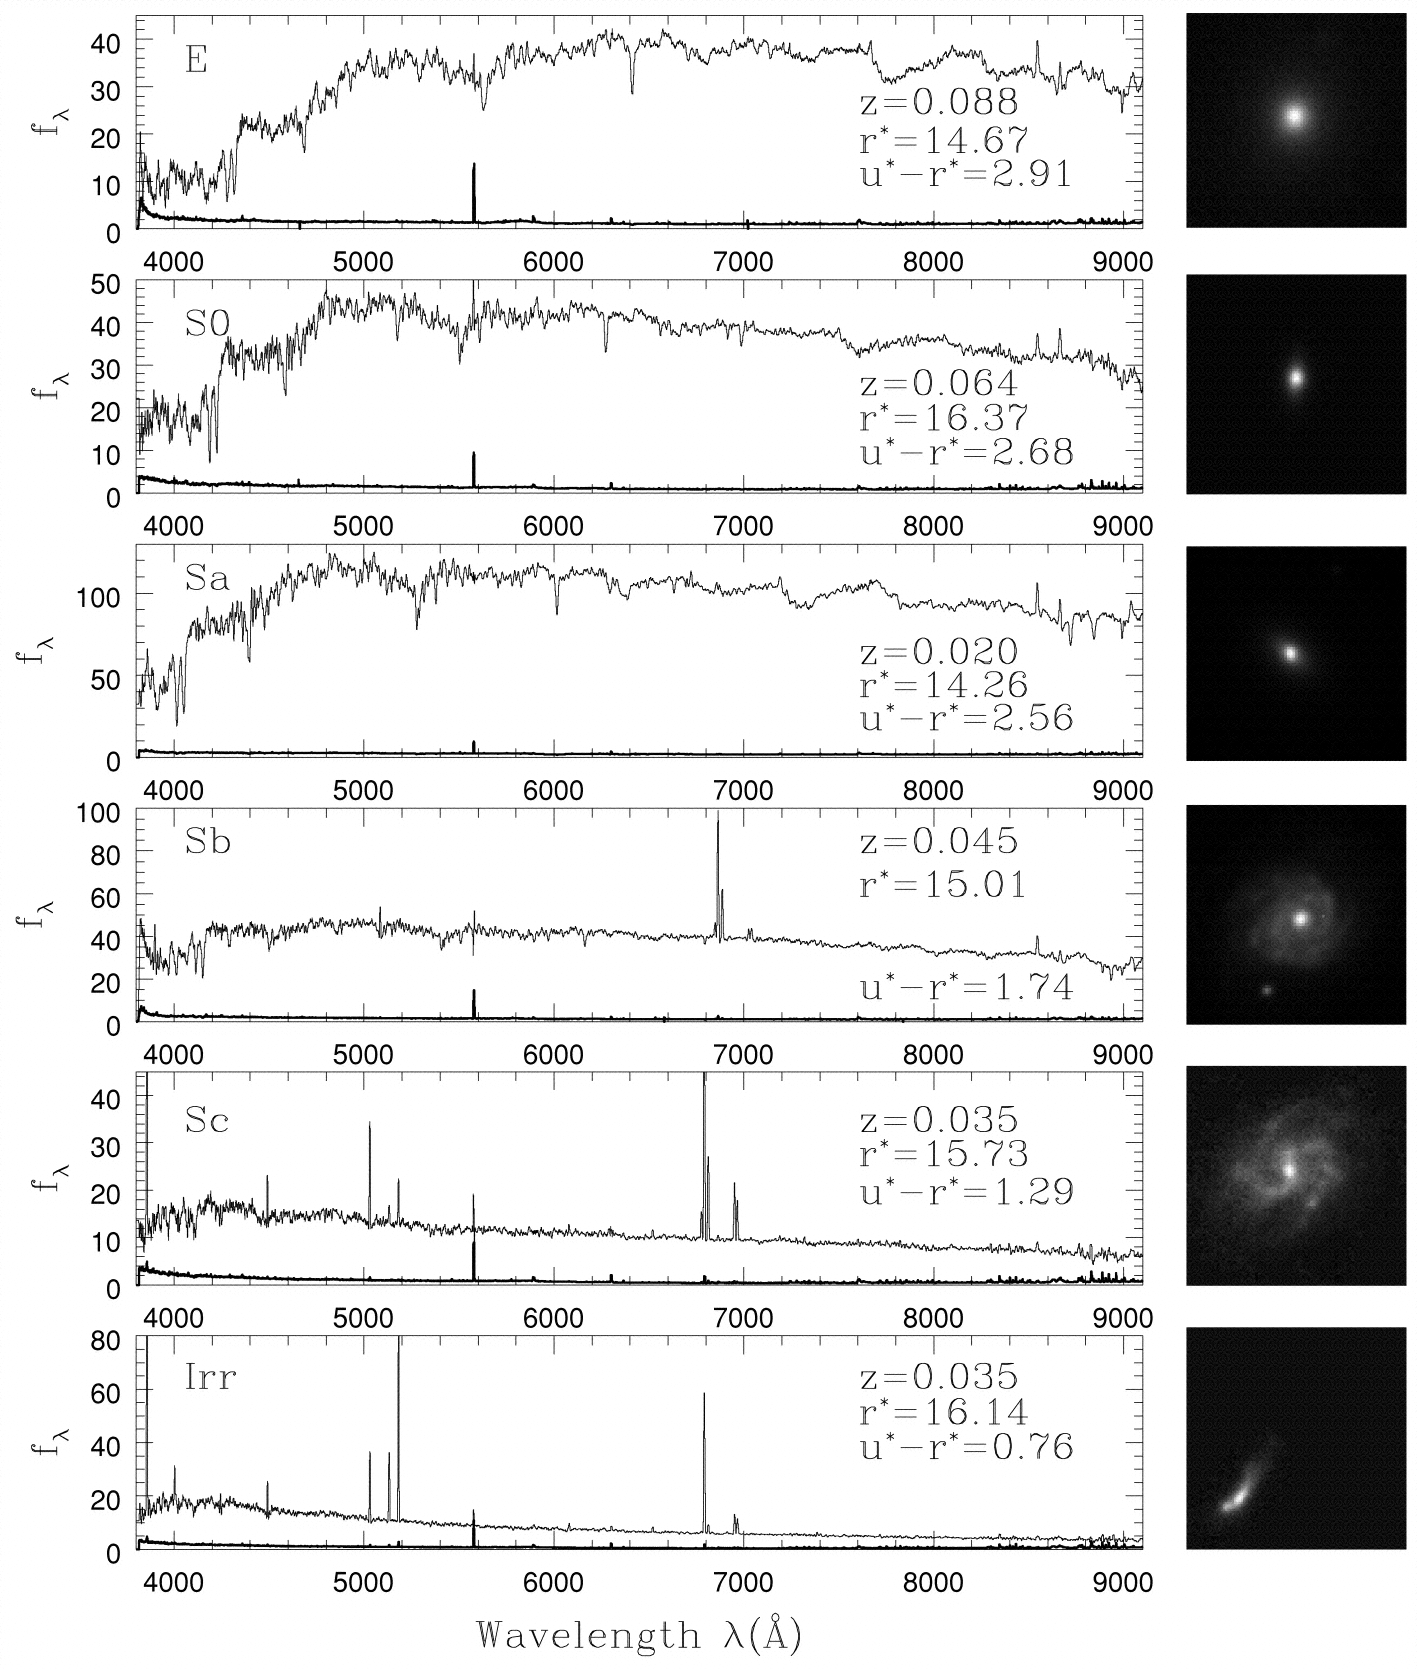
\includegraphics{figures/Strateva_fg4.jpg}}

\end{center}
\end{minipage}

\begin{minipage}[t]{11.5cm}

\begin{itemize}
\item
{\large \color{blue} Spectra are correlated with morphology}
\item
{\large \color{red} Principal component analysis:} spectra form a low-dimensional family:
it is possible to describe most of variance using only 2 parameters (Yip et al. 2004)
\end{itemize}  

\end{minipage}}
\vfill 
\end{slide}
%------------------------------------------------------------------------------


%------------------------------------------------------------------------------
% TWO-SIDED PAGE 
\begin{slide}

\hbox to \hsize{
\begin{minipage}[t]{13cm}
\begin{center}
\vskip 0.1in
\scalebox{0.65}{\hskip -1.5in 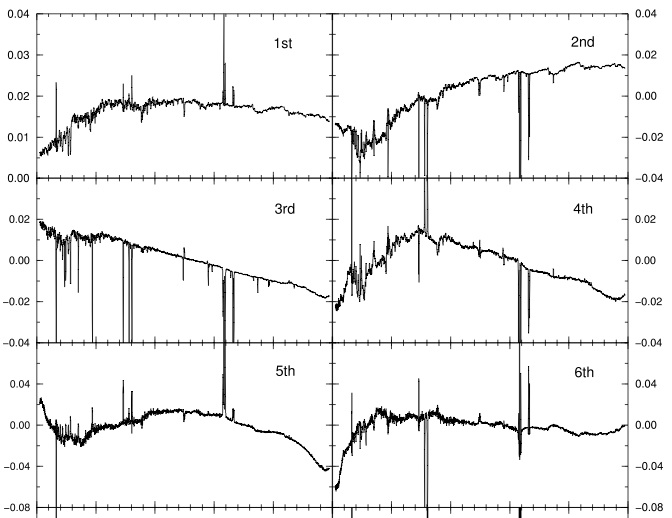
\includegraphics{figures/YipFig1.jpg}}

\end{center}
\end{minipage}

\begin{minipage}[t]{11.5cm}

\begin{itemize}
\item
{\large \color{blue} Spectra are correlated with morphology}
%\item
%{\large \color{red} Principal component analysis:} spectra form a low-dimensional family:
%it is possible to describe most of variance using only 2 parameters (Yip et al. 2004)
{\large \color{red} Principal component analysis:} eigenspectra can be non-negative, which
is not physical; there are other mathematical methods, such as non-negative matrix factorization
(also, non-linear methods known as manifold learning, e.g. locally linear embedding and isometric
mapping), see astroML for code. 
\end{itemize}  

\end{minipage}}
\vfill 
\end{slide}
%------------------------------------------------------------------------------


%------------------------------------------------------------------------------
% TWO-SIDED PAGE 
\begin{slide}

\hbox to \hsize{
\begin{minipage}[t]{13cm}
\begin{center}
\vskip 0.1in
\scalebox{0.85}{\hskip -1.6in 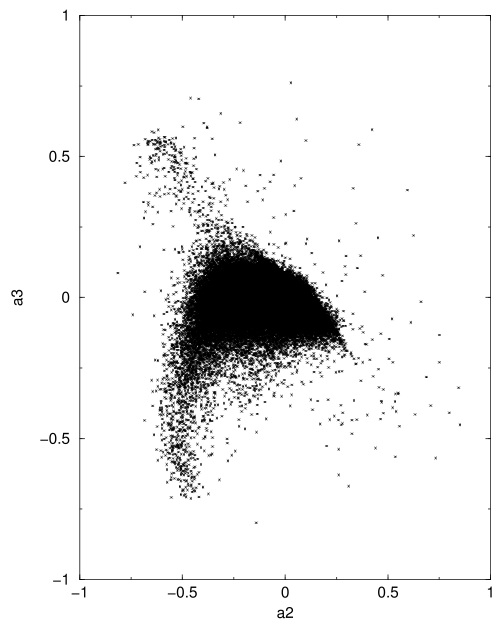
\includegraphics{figures/YipFig2.jpg}}

\end{center}
\end{minipage}

\begin{minipage}[t]{11.5cm}

\begin{itemize}
\item
{\large \color{blue} Spectra are correlated with morphology}
\item
{\large \color{red} Principal component analysis:} spectra form a low-dimensional family:
it is possible to describe most of variance using only 2 parameters (Yip et al. 2004)
\item
{\large \color{blue} What physical quantities can we extract from SDSS spectra of galaxies? }
\end{itemize}  

\end{minipage}}
\vfill 
\end{slide}
%------------------------------------------------------------------------------




%------------------------------------------------------------------------------
% TWO-SIDED PAGE 
\begin{slide}

\hbox to \hsize{
\begin{minipage}[t]{9cm}
\begin{center}
\vskip -0.1in
\scalebox{0.75}{\hskip -1.1in 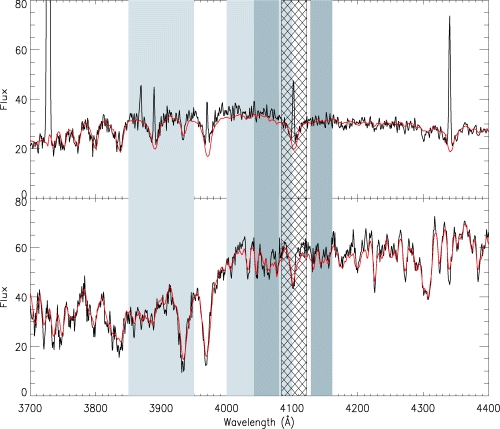
\includegraphics{figures/mnr_6291_f1.jpg}}
\vskip 0.6in
\scalebox{0.75}{\hskip -1.1in 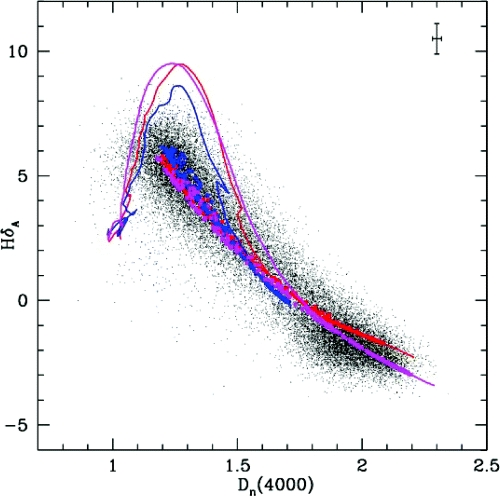
\includegraphics{figures/mnr_6291_f3.jpg}}
\end{center}
\end{minipage}

\begin{minipage}[t]{15cm}
\begin{center}
{\large \color{red} Spectral analysis}
\end{center}

\begin{itemize}
\item
Kauffmann et al. (2003, 2004): model-dependent estimates of {\color{blue} 
stellar mass and dust content using $H_\delta$, $D_{4000}$ and broad-band colors}
\item
{\color{red} From the position in the $H_\delta$ -- $D_{4000}$ diagram, get a model-dependent 
estimate of stellar mass-to-light ratio, and using measured luminosity get stellar
mass.} The measured luminosity is corrected for the dust extinction estimated from 
the discrepancy between the model-predicted and measured broad-band colors.
\end{itemize}  

\end{minipage}}
\vfill 
\end{slide}
%------------------------------------------------------------------------------



%---------------------------------------------------------------------------
% TWO-SIDED PAGE 
\begin{slide}

\hbox to \hsize{
\begin{minipage}[t]{9cm}
\begin{center}
\vskip -0.8in
\scalebox{0.65}{\hskip -1.5in 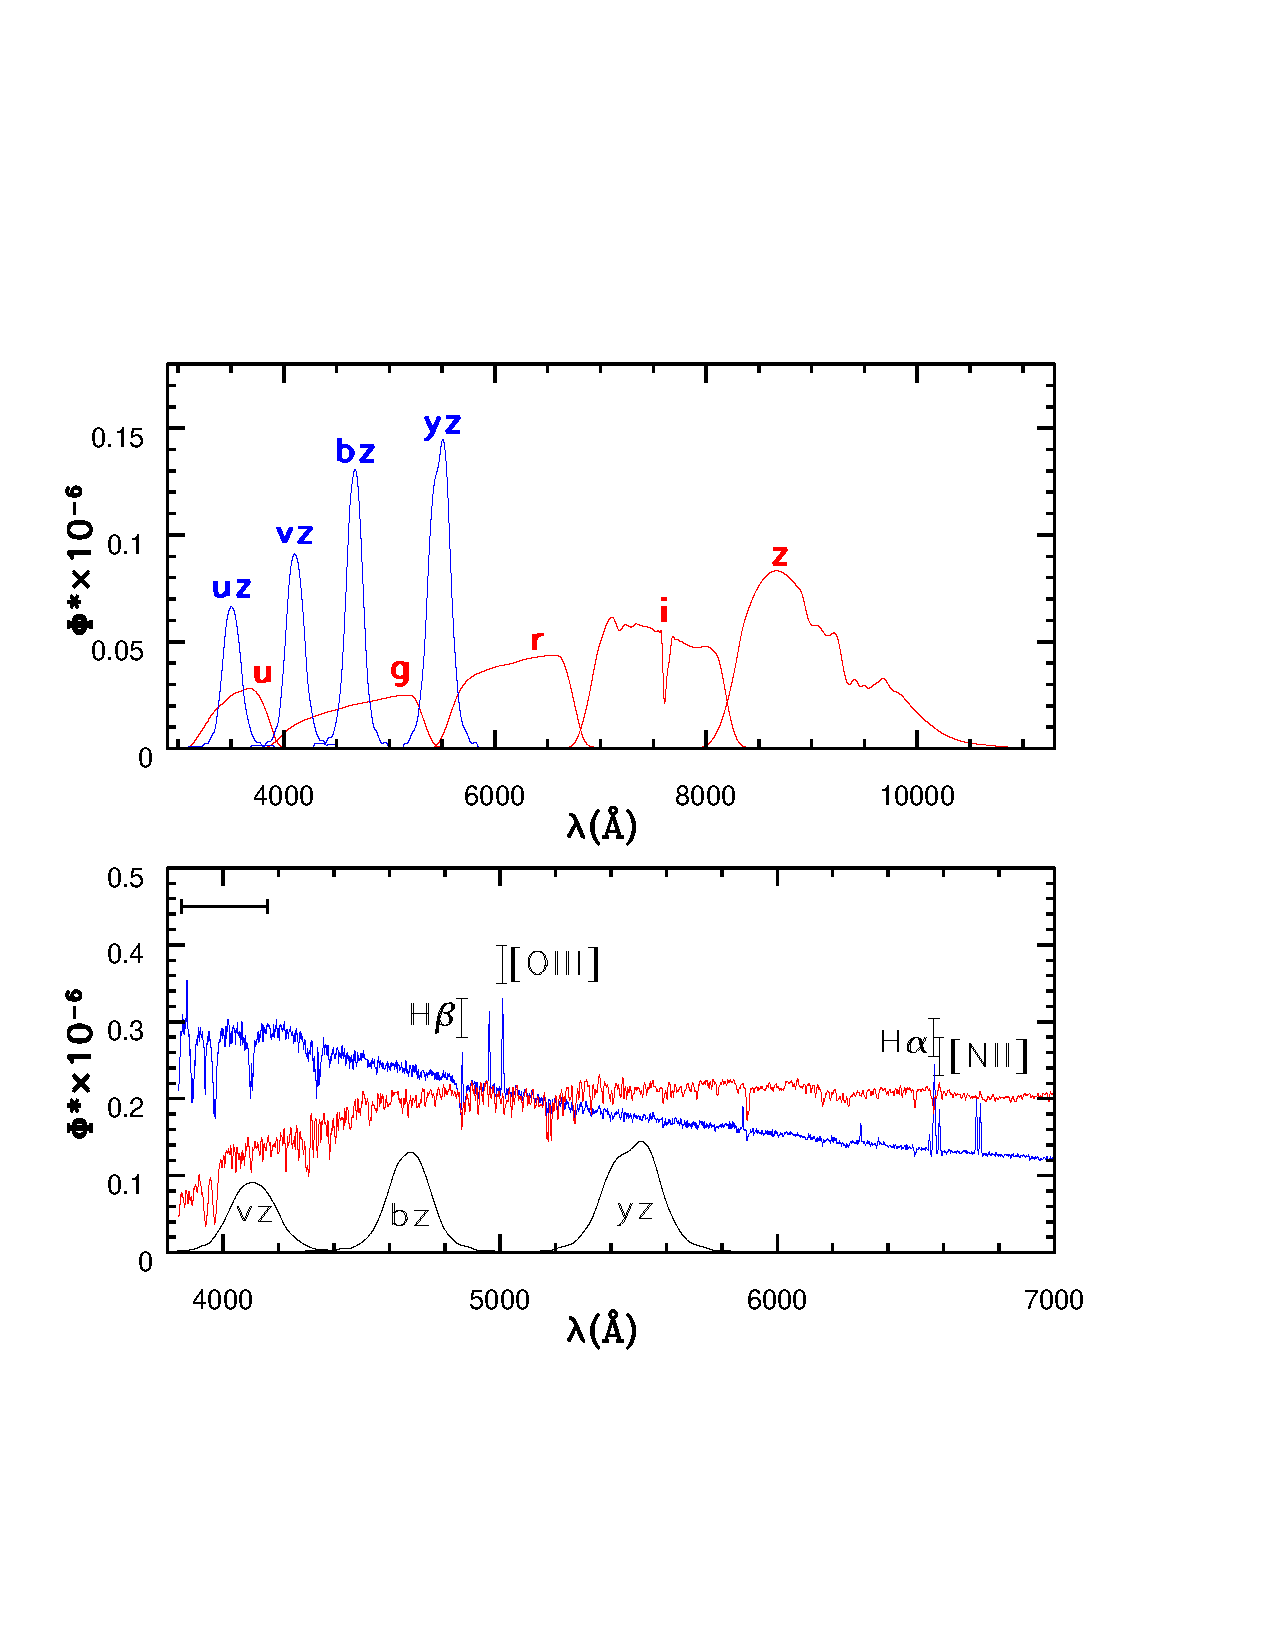
\includegraphics{figures/FltsPlot.pdf}}
\end{center}
\end{minipage}

\begin{minipage}[t]{15cm}
\begin{center}
\vskip -1in
{\large \color{red} Narrow-band rest-frame colors of galaxies in SDSS}
\end{center}

\begin{itemize}
\item
Str\"omgren colors: designed for estimating effective temperature,
metallicity and gravity for stars; narrow band (200 \AA)
\item
SDSS spectra can be used to synthesize narrow-band rest-frame 
colors for galaxies
\item 
{\color{blue} Can we determine age and metallicity of galaxies?}
\end{itemize}  

\end{minipage}}
\vfill 
\end{slide}
%------------------------------------------------------------------------------


%---------------------------------------------------------------------------
% TWO-SIDED PAGE 
\begin{slide}

\hbox to \hsize{
\begin{minipage}[t]{9cm}
\begin{center}
\vskip 0.3in
\scalebox{0.4}{\hskip -1.9in 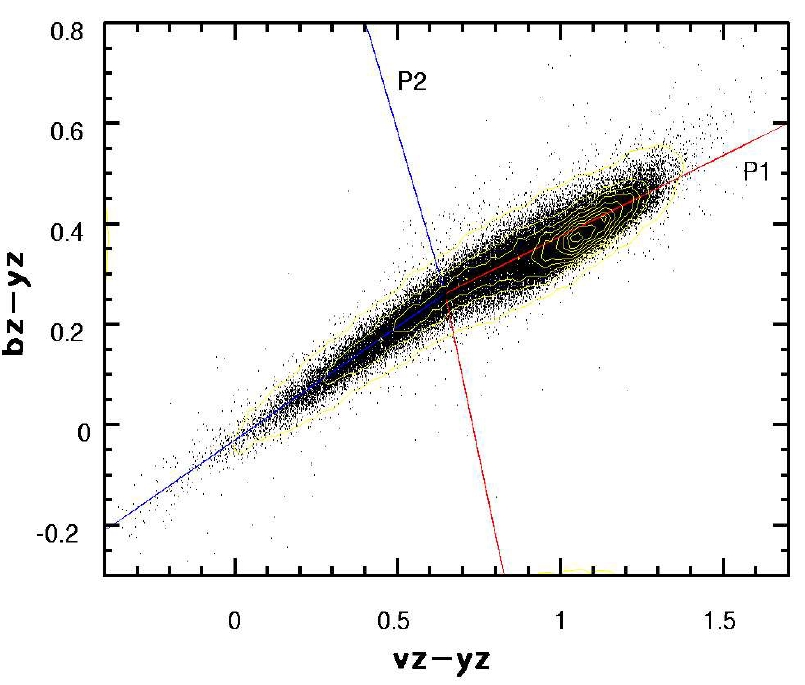
\includegraphics{figures/by_vy.jpg}}
\vskip -1.5in
\scalebox{0.6}{\hskip -1.5in 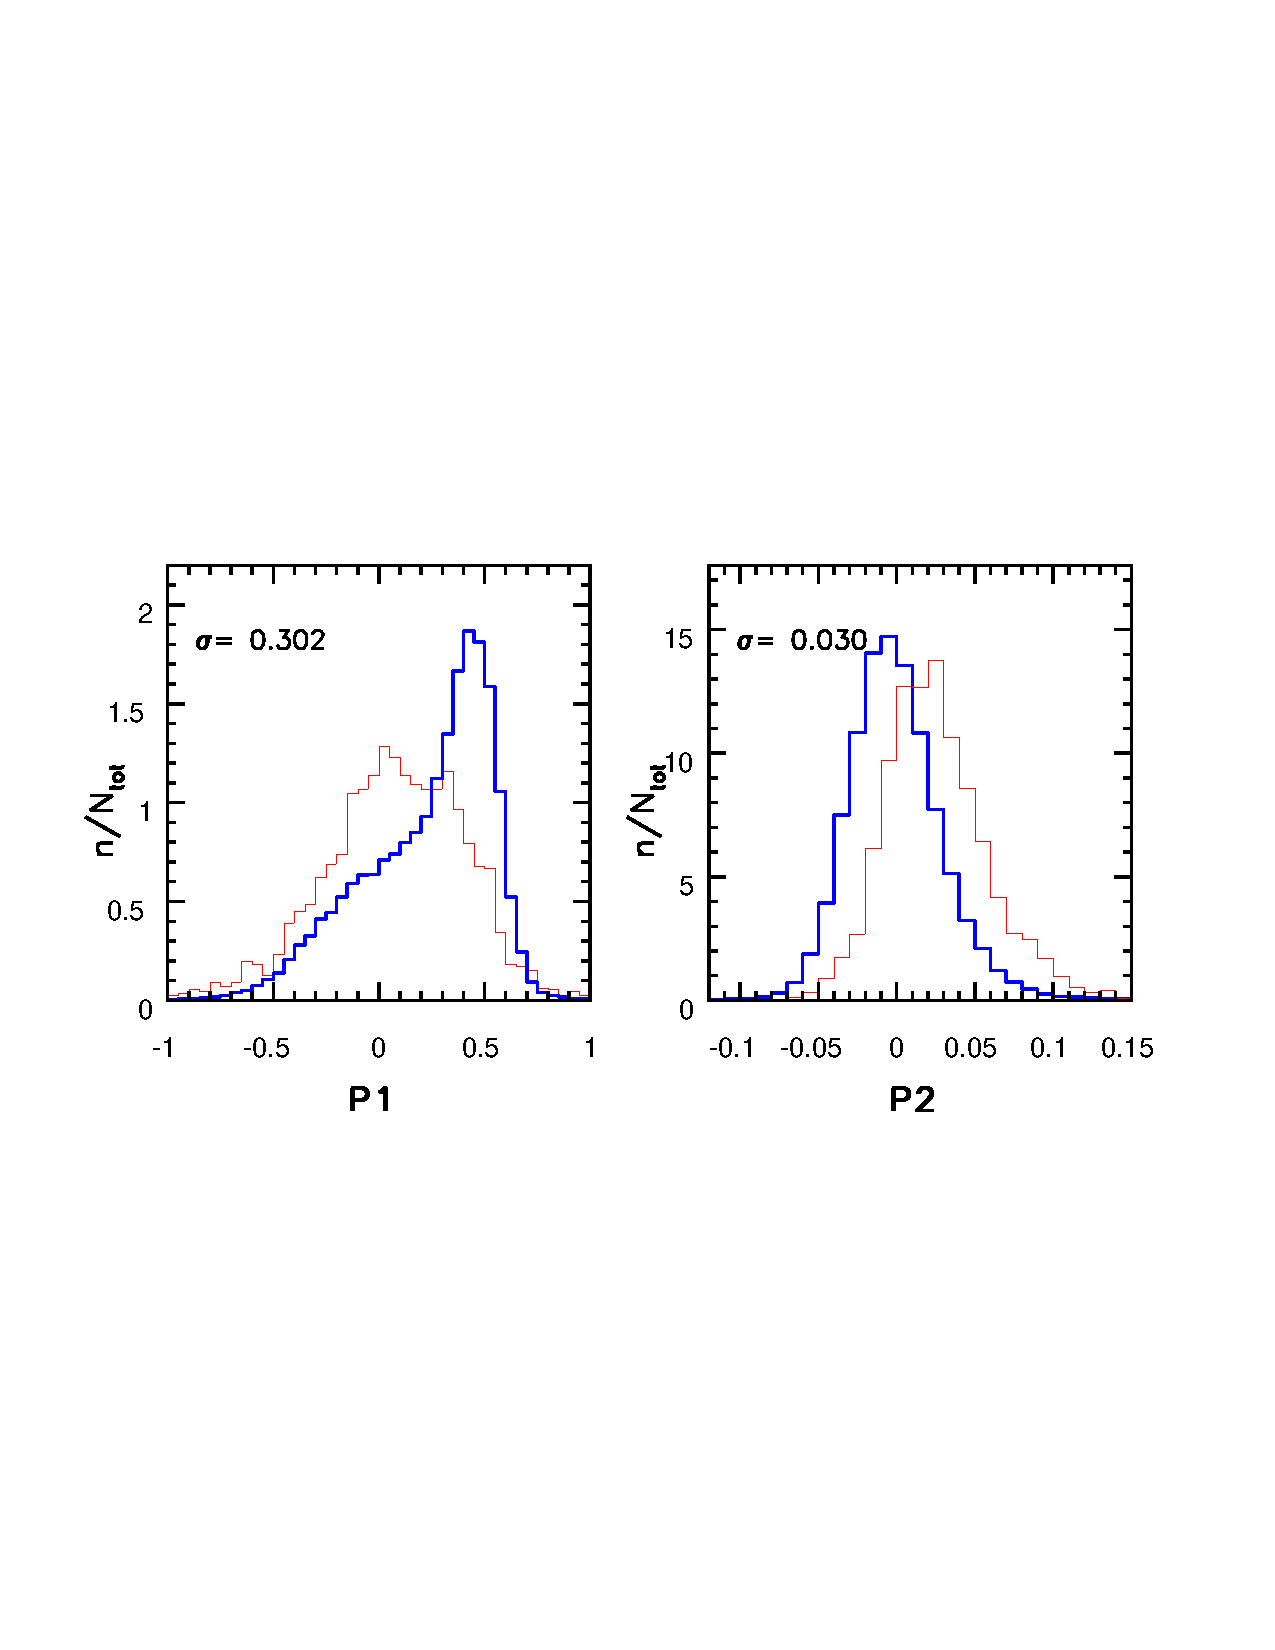
\includegraphics{figures/P1P2hist.pdf}}

\end{center}
\end{minipage}

\begin{minipage}[t]{15cm}
\begin{center}
\vskip -1in
{\large \color{red} Narrow-band rest-frame colors of galaxies in SDSS}
\end{center}

\begin{itemize}
\item
{\color{blue} Galaxies form a narrow locus in rest-frame colors}: SEDs are nearly a
one-dimensional family, with the Hubble type controlling the position
along the locus (Smol\v{c}i\'{c} et al. 2006, MNRAS 371, 121)
\item 
The locus width is only 0.03 mag; the offset in the ``narrow'' direction
is correlated with the dust content
\item
In order to demonstrate that this width is only 0.03 mag, an accurate survey
such as SDSS was needed!
\end{itemize}  
\vskip 0.05in
\scalebox{0.35}{\hskip 1.0in 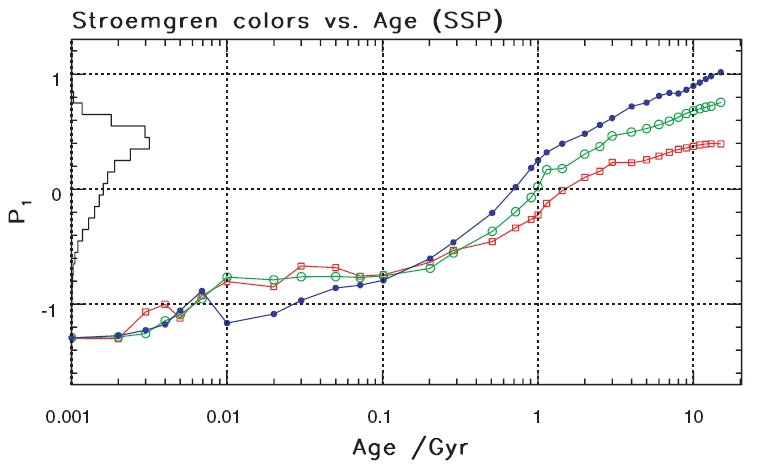
\includegraphics{figures/Smolcic_fig8a.jpg}}
\end{minipage}}
\vfill 
\end{slide}
%------------------------------------------------------------------------------



%---------------------------------------------------------------------------
% TWO-SIDED PAGE 
\begin{slide}

\hbox to \hsize{
\begin{minipage}[t]{9cm}
\begin{center}
\vskip -0.5in
\scalebox{0.75}{\hskip -1.5in 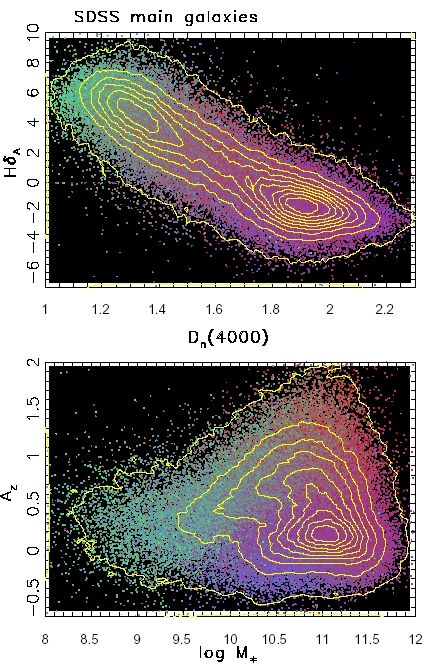
\includegraphics{figures/HdDtotal.jpg}}
\end{center}
\end{minipage}

\begin{minipage}[t]{15cm}
\begin{center}
\vskip -1in
{\large \color{red}   Narrow-band rest-frame colors of galaxies in SDSS}
\end{center}

\begin{itemize}
\item Left: color-coded by P1 from the previous page
\item
Many observables are correlated! 
\item
E.g. the rest-frame colors with the position in the $H_\delta$ -- $D_{4000}$ diagram
\item
This implies: galaxy mass and colors are well correlated -- the bimodal distribution
in colors reflects a characteristic galaxy mass (stars only): $\sim3\times10^{10}$ M$_\odot$. 
\item This characteristic galaxy mass probably marks the transition between different
physical processes that control galaxy formation and evolution
\end{itemize}  

\end{minipage}}
\vfill 
\end{slide}
%------------------------------------------------------------------------------




%---------------------------------------------------------------------------
% TWO-SIDED PAGE 
\begin{slide}

\hbox to \hsize{
\begin{minipage}[t]{9cm}
\begin{center}
\vskip 0.1in
\scalebox{0.75}{\hskip -1.4in 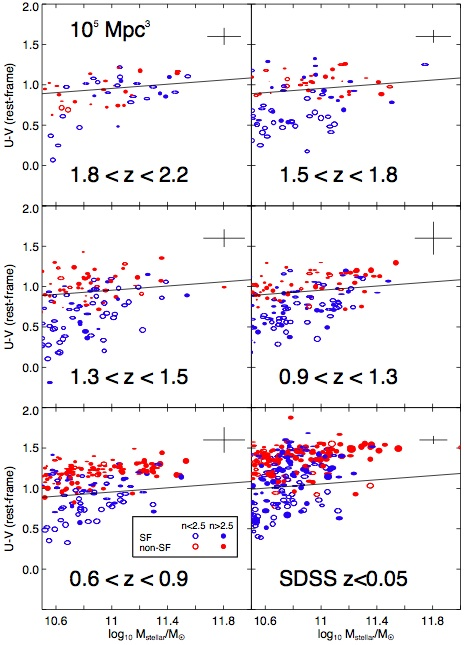
\includegraphics{figures/Bell2012.jpg}}
\end{center}
\end{minipage}

\begin{minipage}[t]{15cm}
\begin{center}
\vskip -1in
{\large \color{red}   Galaxy Evolution}
\end{center}

\begin{itemize}
\item SDSS observations are essentially a snapshot at $z=0$ (now!). 
\item Bell et al. (2012, ApJ 753, 167):  ``We use HST/WFC3 imaging from the CANDELS Multicycle Treasury 
Survey, in conjunction with the Sloan Digital Sky Survey, to explore the evolution of galactic structure for 
galaxies with stellar masses $>3e10 \, M_{sun}$ from $z=2.2$ to the present epoch, a time span of 10 Gyr. 
We explore the relationship between rest-frame optical color, stellar mass, star formation activity and galaxy 
structure.''
\item Left: (fig. 4): The evolution of $U-V$ rest-frame color as a function of stellar mass, 
in redshift bins (the symbol size scales with observed galaxy size, and are color-coded by
star-formation: quiescent galaxies are red). 
\end{itemize}  

\end{minipage}}
\vfill 
\end{slide}
%------------------------------------------------------------------------------


%------------------------------------------------------------------------------
\begin{slide}

\vskip -1.8in
\begin{itemize}
\item
{{\color{red} Morphology-density relation:}} red elliptical galaxies are found in regions more populated by galaxies than
blue spiral galaxies (Dressler 1980, ApJ 236, 351; Postman \& Geller 1984, ApJ 281, 95)
\item
SDSS-based visualization (Cowan \& Ivezi\'{c} 2008, ApJ 674, L13): 
\end{itemize}

\vskip -0.8in
\phantom{x}
\scalebox{0.62}{\hskip 1.4in 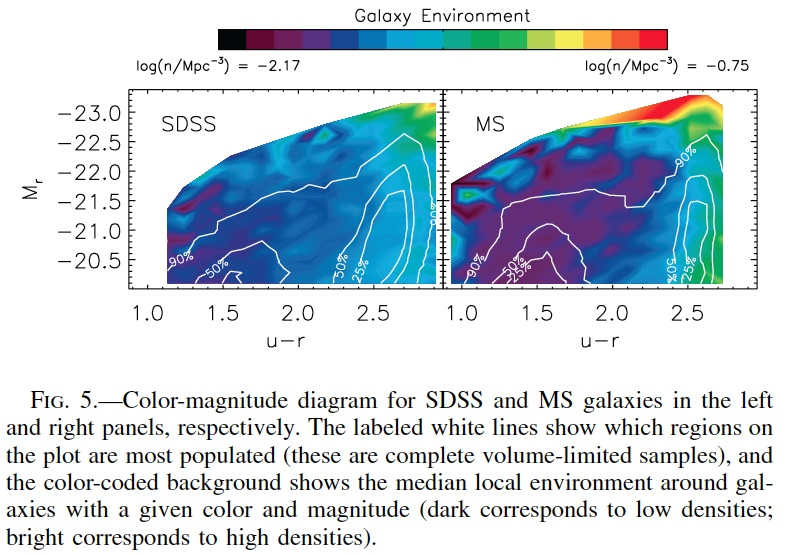
\includegraphics{figures/CowanIvezic.jpg}}

\vfill
\end{slide}
 
%------------------------------------------------------------------------------
% TWO-SIDED PAGE 
\begin{slide}

\hbox to \hsize{
\begin{minipage}[t]{12cm}
\begin{center}
\vskip 0.4in
\scalebox{0.6}{\hskip -1.4in 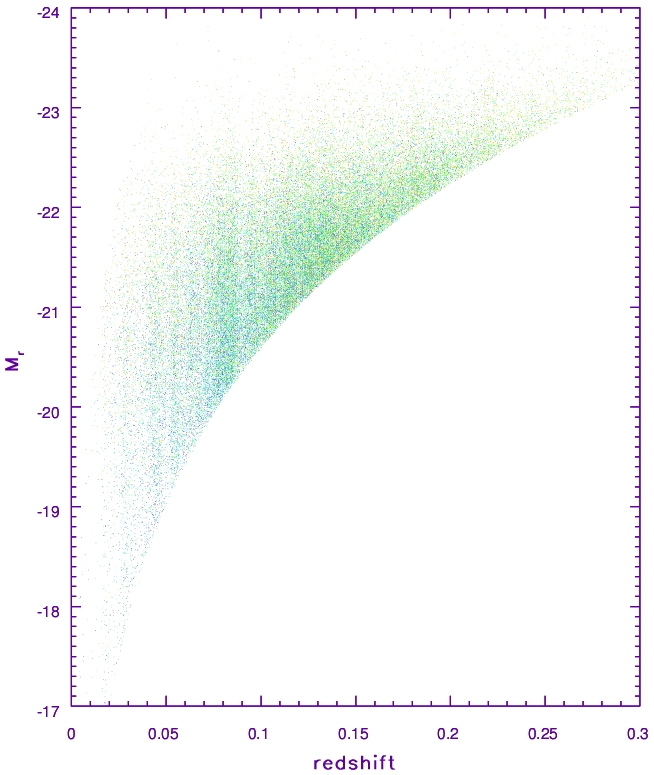
\includegraphics{figures/galLF.jpg}}
\vskip -2in
{\color{red} 
$ p(M,z) = {1 \over N} \Psi(M,z) {dV \over dz} s(M,z,..) $
}
\end{center}
\end{minipage}

\begin{minipage}[t]{12cm}
\begin{center}
\vskip -1in
{\large \color{red} Luminosity Function}
\end{center}

\begin{itemize}
\item {\colour{blue} Luminosity Function is the distribution in the luminosity--position plane;
how many galaxies per unit interval in luminosity and unit volume (or redshift):} {\color{red} $\Psi(M,z)$}
\item Imagine a tiny area with the widths $\Delta Mr$ and $\Delta z$  centered at some $Mr$ and $z$ 
in the plot to the left: count the number of galaxies, divide by $\Delta Mr
\Delta z$, correct for the fraction of sky covered by your survey, and for
the selection probability (a function of $Mr$, $z$, and possibly many other
parameters): this gives you $\Psi(M,z)$.
\end{itemize}  

\end{minipage}}
\vfill 
\end{slide}
%------------------------------------------------------------------------------






%------------------------------------------------------------------------------
\begin{slide}
\begin{center}
\bfseries
{\large {\color{red} Luminosity Function}}
\end{center}
\vskip 0.2in
\hrule


\begin{itemize}
\item {\colour{blue} Luminosity Function is the distribution in the luminosity--position plane;
how many galaxies per unit interval in luminosity and unit volume:} $\Psi(M,z)$
\item
Often, this is a separable function: $\Psi(M,z) = \Phi(M) \, n(z)$, where $\Phi(M)$ is the
absolute magnitude (i.e. luminosity) distribution, and $n(z)$ is the number volume density. 
\item Luminosity is a product of flux and distance squared (ignore cosmological
effects for simplicity): {\colour{blue} $L = 4 \pi D^2 F$}
\item
The samples are usually {\it flux-limited} (meaning: all sources brighter than some 
flux limit are detected) -- {\colour{blue} the minimum detectable luminosity depends on distance}:
$L > 4 \pi D^2 F_{min}$, or for absolute magnitude $M < M_{max}(D)$ (c.f. the first plot)

\end{itemize}

\vfill
\end{slide}
 





%------------------------------------------------------------------------------
\begin{slide}
\begin{center}
\bfseries
{\large {\color{red} Schechter Function}}
\end{center}
\vskip 0.2in
\hrule

Galaxy luminosity distribution resembles a power-law, with an exponential
cutoff. This distribution is usually modeled by Schechter function:
\eq{
      \Phi(L)  = \Phi^\ast \, \left({L \over L_\ast}\right)^\alpha {\rm e}^{-L/L_\ast}
}


Or using absolute magnitudes:
\eq{
\Phi(Mr) = 0.4 \Phi^\ast \, {\rm e}^{-0.4(\alpha+1)(Mr-M^\ast)} \, {\rm e}^{-{\rm e}^{-0.4(Mr-M^\ast)}}
}



\vfill
\end{slide}
 

%------------------------------------------------------------------------------
\begin{slide}

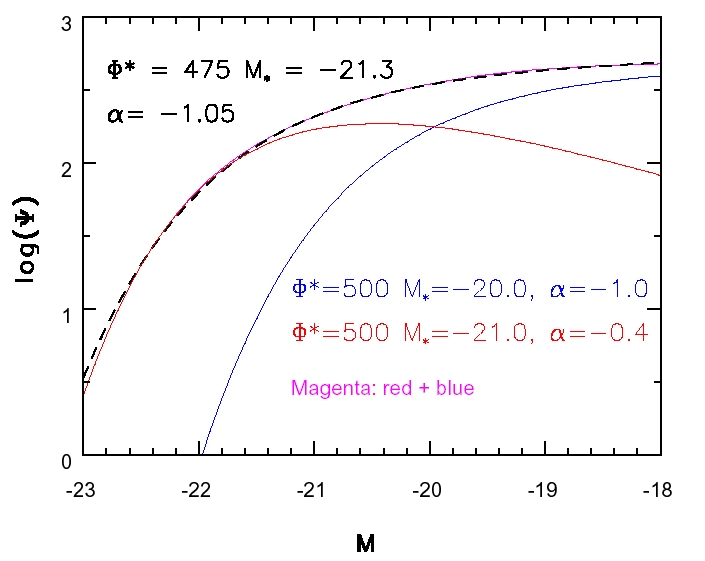
\includegraphics{figures/Schechter.jpg}



\vfill
\end{slide}
 




%------------------------------------------------------------------------------
% TWO-SIDED PAGE 
\begin{slide}

\hbox to \hsize{
\begin{minipage}[t]{12cm}
\begin{center}
\vskip 0.4in
\scalebox{0.6}{\hskip -1.4in 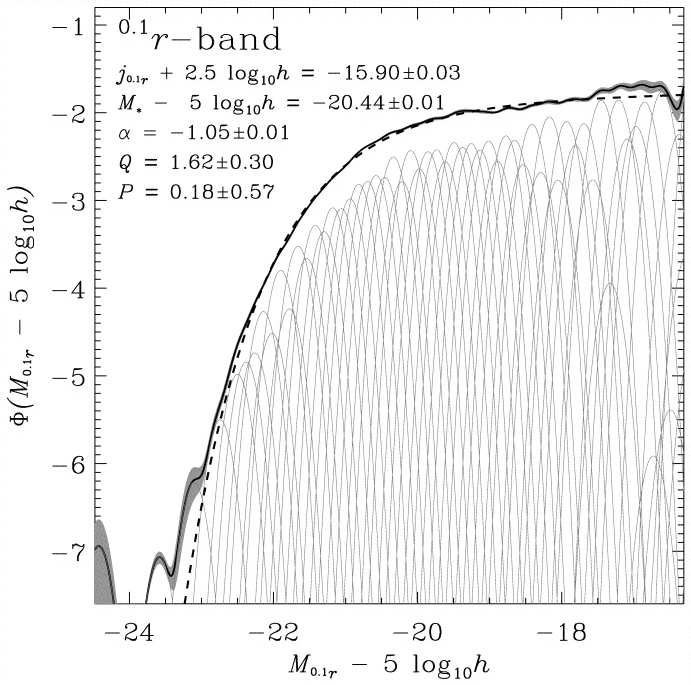
\includegraphics{figures/fg5.jpg}}
Note: this LF cannot be expressed as $\Phi(M,z) = f(M) \, g(z)$ -- not separable!
\end{center}
\end{minipage}

\begin{minipage}[t]{12cm}
\begin{center}
\vskip -1in
{\large \color{red} The LF in the SDSS $r$ band}
\end{center}

\begin{itemize}
\item The thick solid line is the SDSS $r$ band luminosity function,
and the gray band is its uncertainty.
\item
The dashed line is a Schechter-like fit that also includes the effects
of changing luminosity and the number density with time (i.e. distance,
or redshift). $Q > 0$ indicates that galaxies were more 
luminous in the past, and $P>0$ that galaxies were more 
numerous in the past. For detailed discussion, see Blanton
et al. 2003 (Astronomical Journal, 592, 819-838)
\end{itemize}  


\end{minipage}}
\vfill 
\end{slide}
%------------------------------------------------------------------------------


%------------------------------------------------------------------------------
% TWO-SIDED PAGE 
\begin{slide}

\hbox to \hsize{
\begin{minipage}[t]{10cm}
\begin{center}
\vskip -0.6in
\scalebox{0.65}{\hskip -1.6in 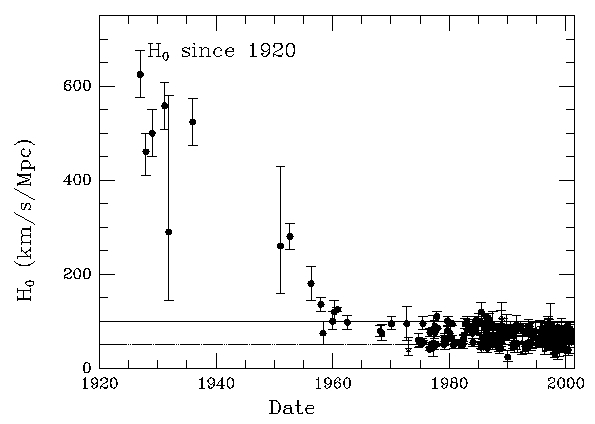
\includegraphics{figures/h1920_2.jpg}}
\vskip -0.2in
\scalebox{0.65}{\hskip -1.7in 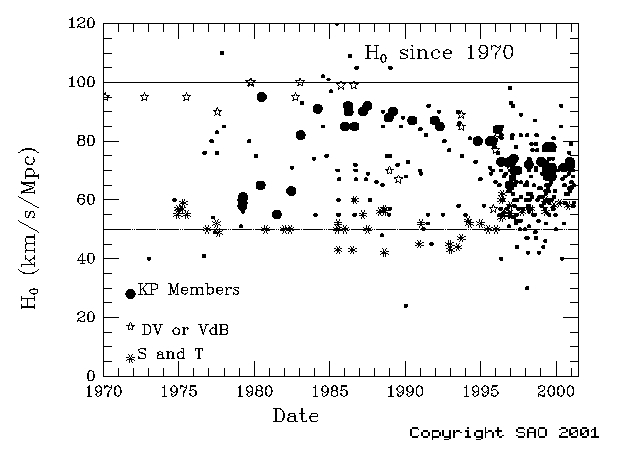
\includegraphics{figures/h1970.jpg}}
\end{center}
\end{minipage}

\begin{minipage}[t]{14cm}
\vskip -1in
\begin{center}
{\large \color{red} $H_o$ as ``a function of time'' }
\end{center}

\begin{itemize}
\item the first three points: Lemaitre (1927), Robertson (1928), Hubble (1929), all 
          based on Hubble's data
\item the early low value (290 km/s/Mpc): Jan Oort
\item the first major revision: discovery of Population II stars by Baade
\item the very recent convergence to values near 65$\pm$10 km/sec/Mpc 
\item the best Cepheid-based value for the local $H_o$ determination is 71$\pm$7 km/s/Mpc,
      the WMAP5 value based on cosmic microwave background measurements: 72$\pm$3 km/s/Mpc. 
\item WMAP9: 69.3$\pm$0.8 km/s/Mpc, and the Planck Mission: {\color{red} $H_o = 67.8 \pm 0.8$ km/s/Mpc}  ($h=0.678$) 
\item Thusly, $-$5log$_{10}$(h) = 0.84 mag! 
\end{itemize}
\end{minipage}}
\vfill 
\end{slide}
%--------------------------------------------------------------------------------------------








%------------------------------------------------------------------------------
% TWO-SIDED PAGE 
\begin{slide}

\hbox to \hsize{
\begin{minipage}[t]{9cm}
\begin{center}
\vskip -0.1in
\scalebox{0.7}{\hskip -1.4in 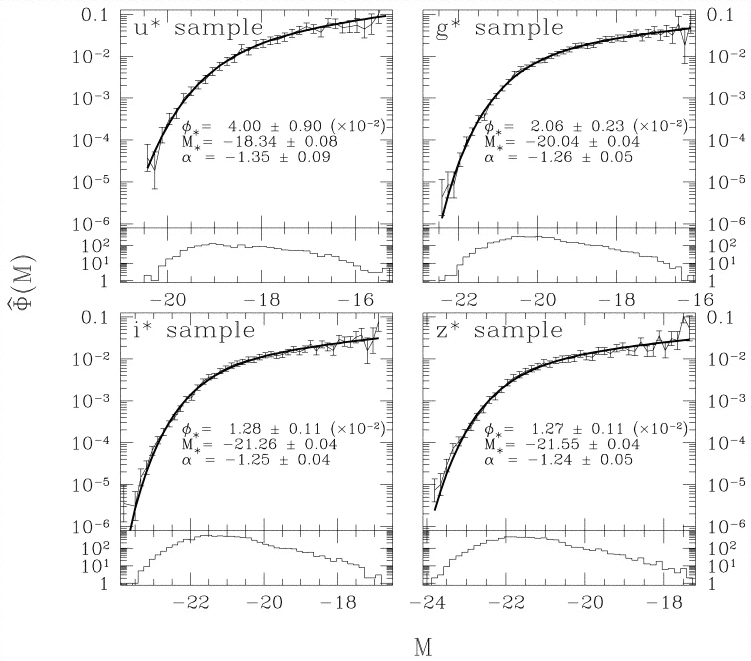
\includegraphics{figures/Blanton_LFs.jpg}}
\vskip 0.1in
\scalebox{0.45}{\hskip -1.3in 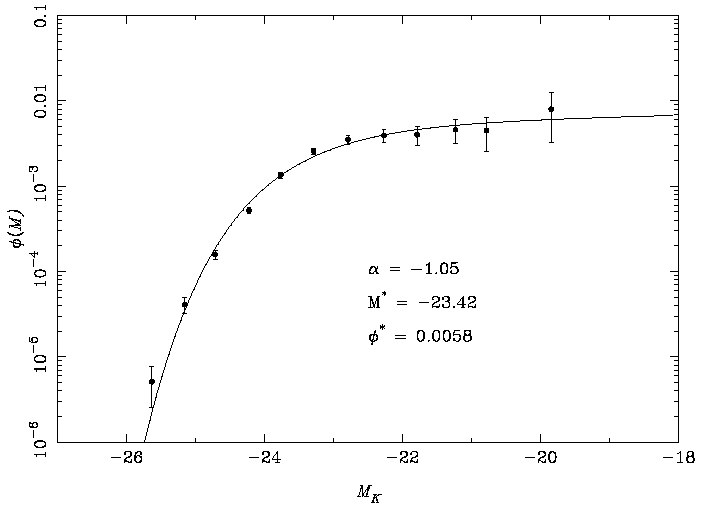
\includegraphics{figures/lf4_K.jpg}}
\end{center}
\end{minipage}

\begin{minipage}[t]{15cm}
\begin{center}
{\large \color{red} The dependence of LF on wavelength}
\end{center}

\begin{itemize}
\item
Top: SDSS ugiz bands
\item
Bottom: 2MASS K band
\item
{\color{blue} The Schechter function is still a good fit, but best-fit parameters vary.} 
\item 
Since the SEDs of galaxies are nearly one-dimensional families,
once the LF for a sample selected by color or morphology is 
known, the LFs at other wavelengths can be simply obtained
by shifting the M axis by the appropriate color difference. 
\item
This doesn't work for the LFs in the top four panels because 
they are computed for the whole sample.
\end{itemize}  

\end{minipage}}
\vfill 
\end{slide}
%------------------------------------------------------------------------------




%------------------------------------------------------------------------------
% TWO-SIDED PAGE 
\begin{slide}

\hbox to \hsize{
\begin{minipage}[t]{9cm}
\begin{center}
\vskip -0.1in
\scalebox{0.7}{\hskip -1.4in 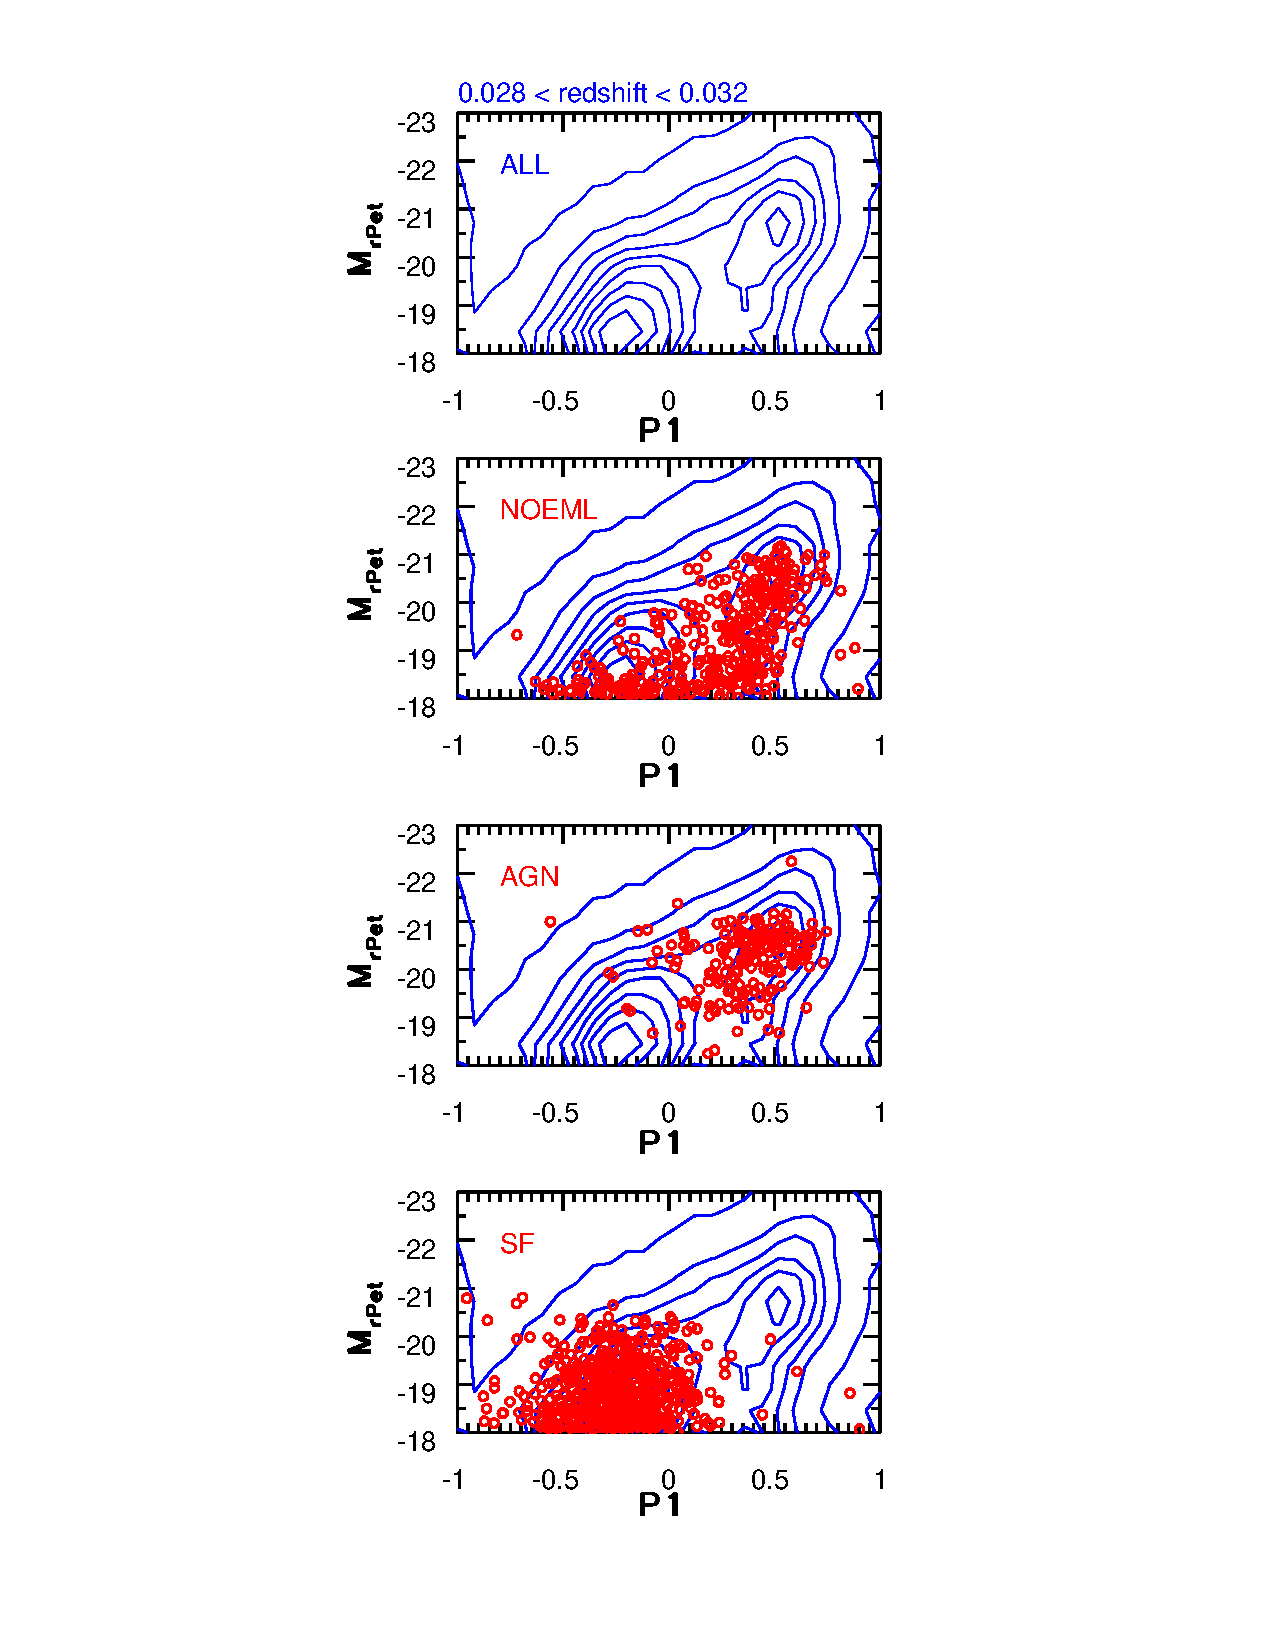
\includegraphics{figures/plotMrPetP1.pdf}}
\end{center}
\end{minipage}

\begin{minipage}[t]{15cm}
\begin{center}
{\large \color{red} The dependence of LF on galaxy type}
\end{center}


\begin{itemize}
\item
The top panel shows the distribution of SDSS galaxies in the 
absolute magnitude -- color plane (in a narrow redshift range)
\item
In the bottom three panels, the same distribution is compared to
the distributions for subsamples selected by their emission
line properties
\item
Note that the most luminous galaxies ($M_r < -20$) are predominantly
red ($P1 > 0.2$), while faint galaxies  ($M_r > -19$) are blue ($P1 < 0.2$) 
\end{itemize}  


\end{minipage}}
\vfill 
\end{slide}
%------------------------------------------------------------------------------




%------------------------------------------------------------------------------
% TWO-SIDED PAGE 
\begin{slide}

\hbox to \hsize{
\begin{minipage}[t]{9cm}
\begin{center}
\vskip 0.4in
\scalebox{0.65}{\hskip -1.4in 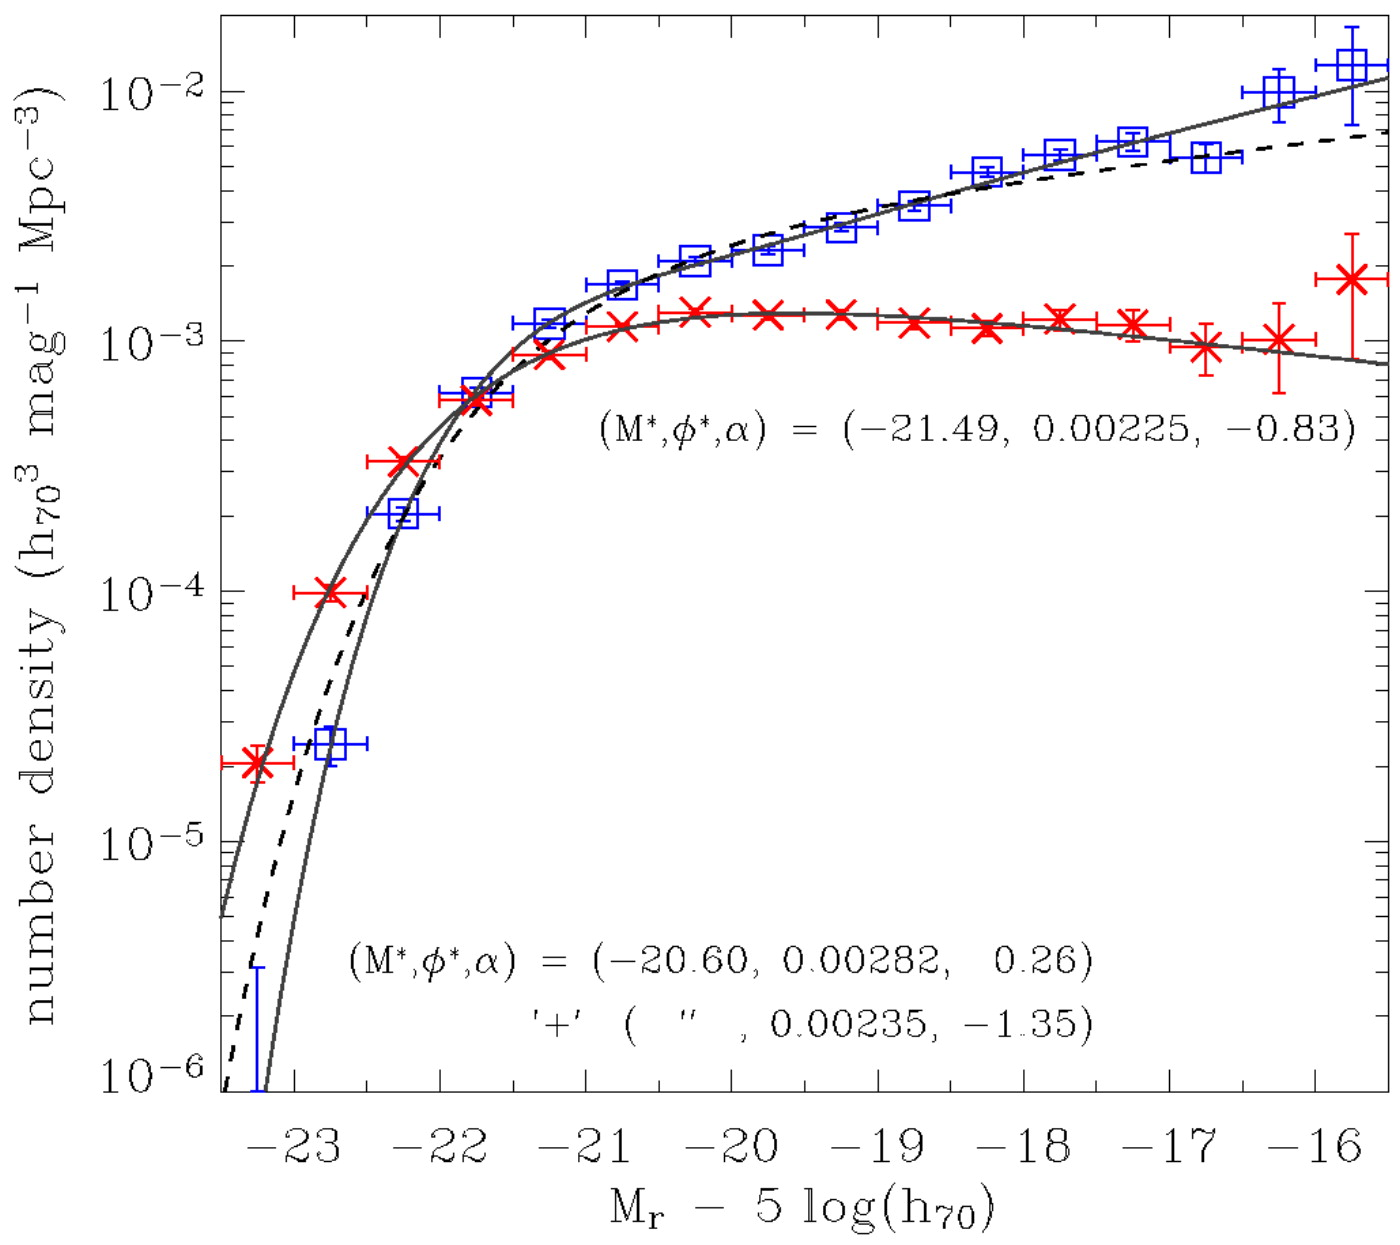
\includegraphics{figures/LFtype.jpg}}
\end{center}
\end{minipage}

\begin{minipage}[t]{15cm}
\begin{center}
{\large \color{red} The dependence of LF on galaxy type}
\end{center}


\begin{itemize}
\item
The comparison of LFs for blue and red galaxies (from Baldry 
et al. 2004, ApJ, 600, 681-694)
\item
The red distribution has a more luminous characteristic magnitude 
and a shallower faint-end slope, compared to the blue distribution
\item
The transition between the two types corresponds to stellar mass
of $\sim3\times10^{10}$ M$_\odot$ 
\item
The differences between the two LFs are consistent with the red 
distribution being formed from major galaxy mergers.
\end{itemize}  


\end{minipage}}
\vfill 
\end{slide}
%------------------------------------------------------------------------------


%------------------------------------------------------------------------------
\begin{slide}
\begin{center}
\bfseries
{\large {\color{red} The C$^-$ method for estimating LF}}
\end{center}
\vskip 0.2in
\hrule

\begin{itemize}
\item Lynden-Bell (1971, MNRAS 155, 95); a non-parametric method that works 
for separable LFs, $\Psi(L,z) = \Phi(L) n(z)$
\item practically all non-parametric methods can be reduced to the $C^-$
      method (Petrosian 1992)
\item parametric methods are usually based on maximizing likelihood
      (e.g. Marshall 1985)
\item the simplest and most famous method, the $V_{max}$ method (Schmidt 1968),
      requires binning in two axes simultaneously, while with the $C^-$
      method data is binned only one axis at a time (e.g. Fan et al. 2001) 
\item How do we know that separable LF is a good guess for our data?
\end{itemize}

\vfill
\end{slide}
 




%------------------------------------------------------------------------------
\begin{slide}
\begin{center}
\bfseries
{\large {\color{red} C$^-$ method}}
\end{center}
\vskip 0.2in
\hrule

\begin{itemize}
\item
Given a set of measured pairs $(x_i, y_i)$, with 
$i=1 \dots N$, and {\it known} relation $y_{max}(x)$, estimate the two-dimensional
distribution, $n(x,y)$, from which the sample was drawn. Assume that 
measurement errors for both $x$ and $y$ are negligible compared to their observed 
ranges, that $x$ is measured within a range defined by $x_{min}$ and $x_{max}$, 
and that the selection function is 1 for $0 \le y\le y_{max}(x)$ and $x_{min} \le x \le x_{max}$,  
and 0 otherwise.
\end{itemize}

\vskip -0.7in
\phantom{x}
\scalebox{0.9}{\hskip 1.4in 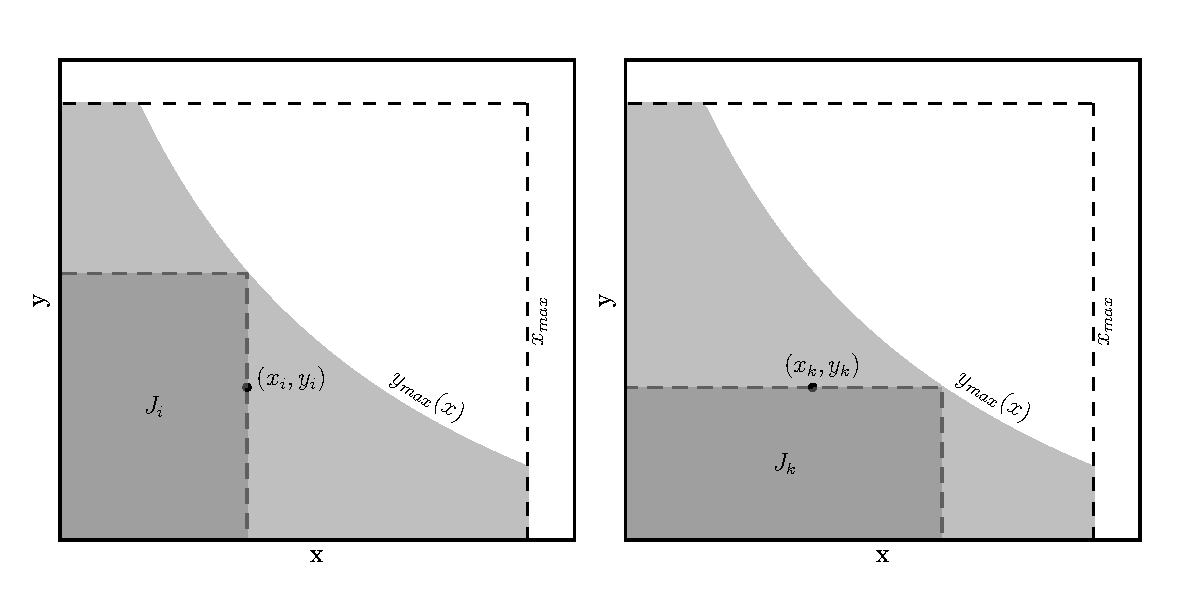
\includegraphics{figures/fig_lyndenbell_setup-1.pdf}}

\vfill
\end{slide}
 

%------------------------------------------------------------------------------
\begin{slide}
\begin{center}
\bfseries
{\large {\color{red} C$^-$ method}}
\end{center}
\vskip 0.2in
\hrule

\begin{itemize}
\item
$C^-$ method is applicable when the distributions along the two coordinates $x$ and $y$ 
are uncorrelated, that is, when we can assume that the bivariate distribution $n(x,y)$ is separable
\eq{
\label{eq:separable2D}
                    n(x,y) = \Psi(x) \, \rho(y). 
}
Therefore, before using the $C^-$ method we need to demonstrate that this
assumption is valid. 
\end{itemize}

\vskip -0.7in
\phantom{x}
\scalebox{0.9}{\hskip 1.4in 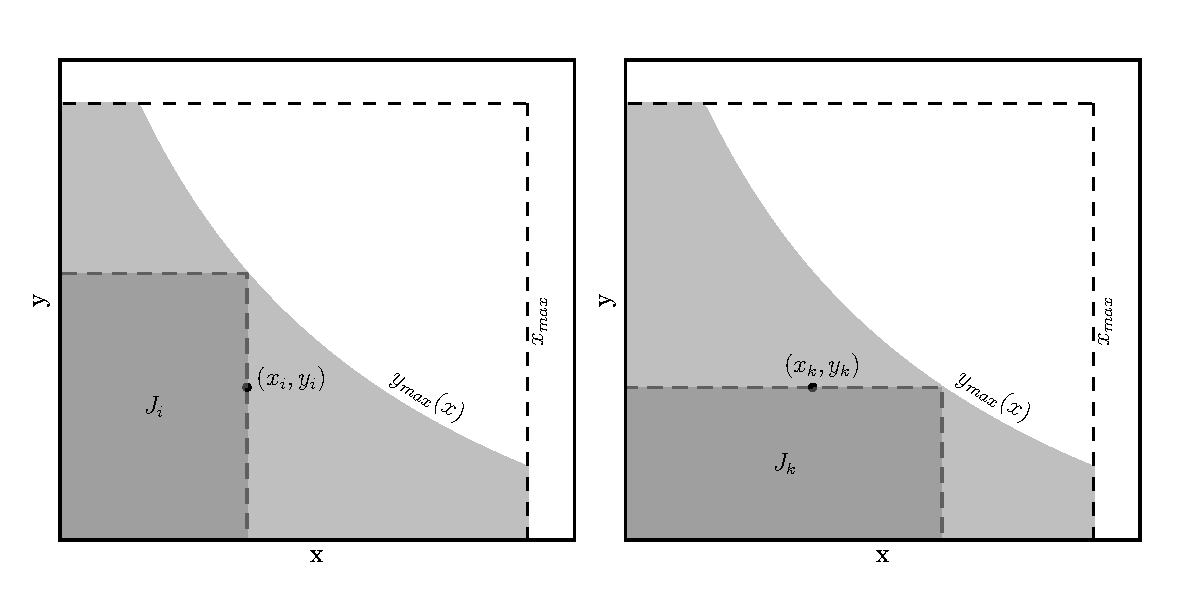
\includegraphics{figures/fig_lyndenbell_setup-1.pdf}}

\vfill
\end{slide}
 

%------------------------------------------------------------------------------
\begin{slide}
\begin{center}
\bfseries
{\large {\color{red} C$^-$ method}}
\end{center}
\vskip 0.2in
\hrule

\begin{itemize}
\item 
Define a {\it comparable} or {\it associated} set for each object $i$ such that 
$J_i = \{ j:x_j < x_i, y_j < y_{max}(x_i)\}$; this is the largest $x$-limited and $y$-limited data 
subset for object $i$, with $N_i$ elements (see the left panel).
\item Sort the set $J_i$ by $y_j$; this gives us the rank $R_j$ for each object (ranging
from 1 to $N_i$)
\end{itemize}

\vskip -0.7in
\phantom{x}
\scalebox{0.9}{\hskip 1.4in 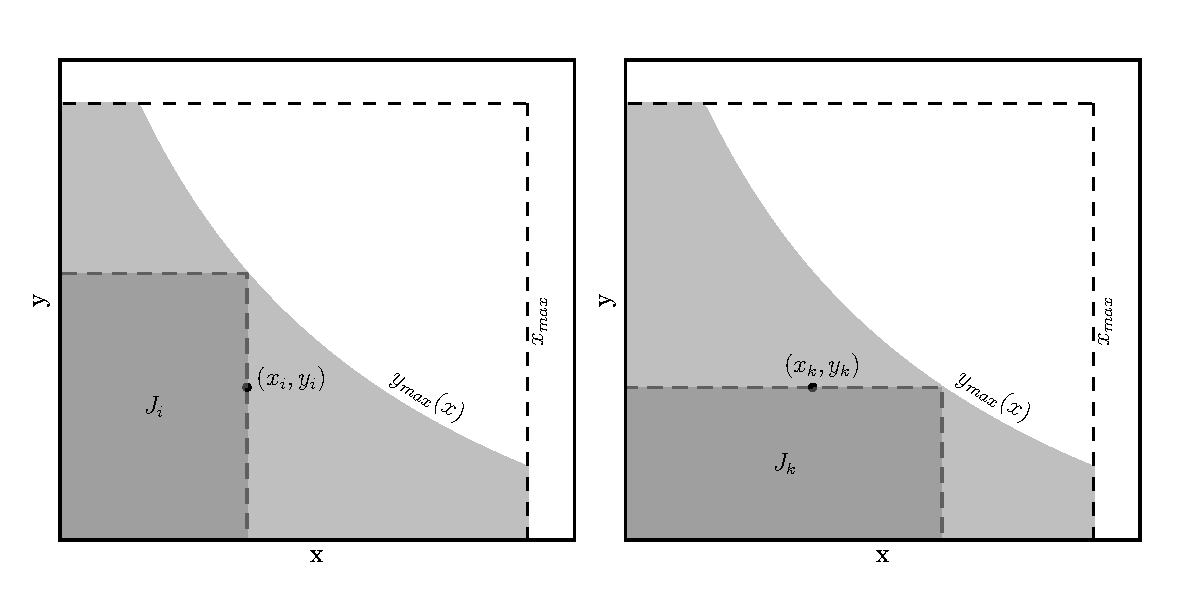
\includegraphics{figures/fig_lyndenbell_setup-1.pdf}}

\vfill
\end{slide}
 

%------------------------------------------------------------------------------
\begin{slide}
\begin{center}
\bfseries
{\large {\color{red} C$^-$ method}}
\end{center}
\vskip 0.2in
\hrule

\begin{itemize}
\item 
Define a {\it comparable} or {\it associated} set for each object $i$ such that 
$J_i = \{ j:x_j < x_i, y_j < y_{max}(x_i)\}$; this is the largest $x$-limited and $y$-limited data 
subset for object $i$, with $N_i$ elements.
\item Sort the set $J_i$ by $y_j$; this gives us the rank $R_j$ for each object (ranging
from 1 to $N_i$)
\item Define the rank $R_i$ for object $i$ in {\it its} associated set: this is 
essentially the number of objects with $y<y_i$ in set $J_i$.
\item If $x$ and $y$ are truly independent, $R_i$ must be distributed 
      {\it uniformly} between 0 and $N_i$. 
\end{itemize}

\vskip -0.7in
\phantom{x}
%\scalebox{0.9}{\hskip 1.4in 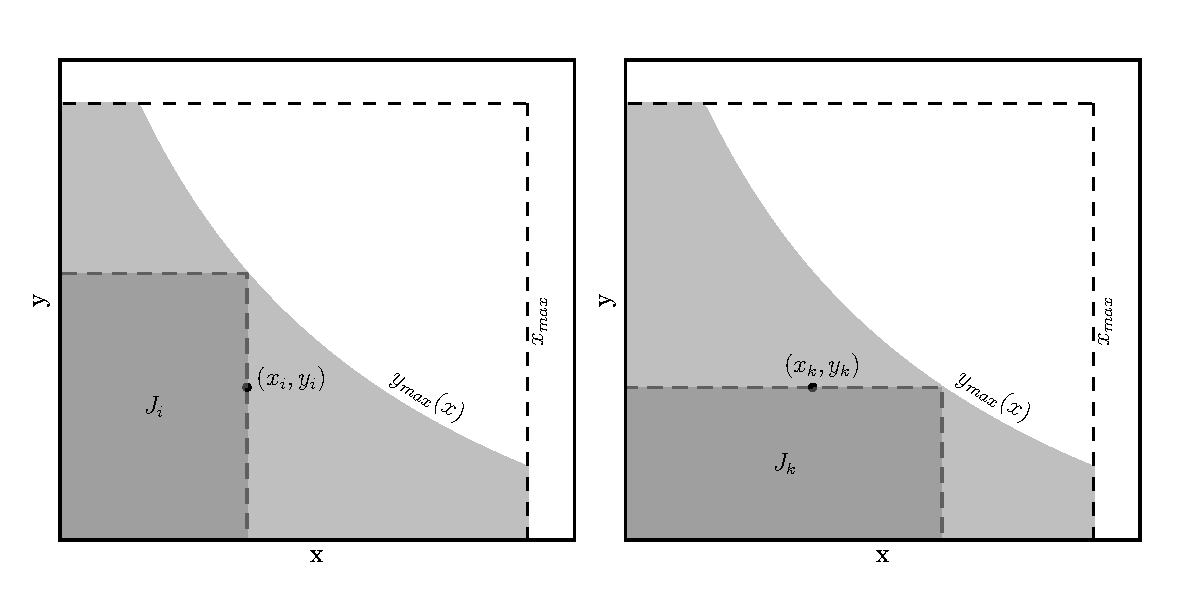
\includegraphics{figures/fig_lyndenbell_setup-1.pdf}}

\vfill
\end{slide}
 


%------------------------------------------------------------------------------
\begin{slide}
\begin{center}
\bfseries
{\large {\color{red} C$^-$ method}}
\end{center}
\vskip 0.2in
\hrule

\begin{itemize}
\item If $x$ and $y$ are truly independent, $R_i$ must be distributed 
      {\it uniformly} between 0 and $N_i$.
\item In this case, it is trivial to determine 
      the expectation value and variance for $R_i$: $E(R_i) = E_i = N_i/2$
      and $V(R_i) = V_i = N_i^2/12$. We can define the statistic
\begin{equation}
      \tau = {\sum_i (R_i - E_i)\over \sqrt {\sum_i V_i   }   } 
\end{equation}
If $\tau < 1$, then $x$ and $y$ are uncorrelated at $\sim1 \sigma$ level! 
\end{itemize}

\vskip -0.7in
\phantom{x}
%\scalebox{0.9}{\hskip 1.4in 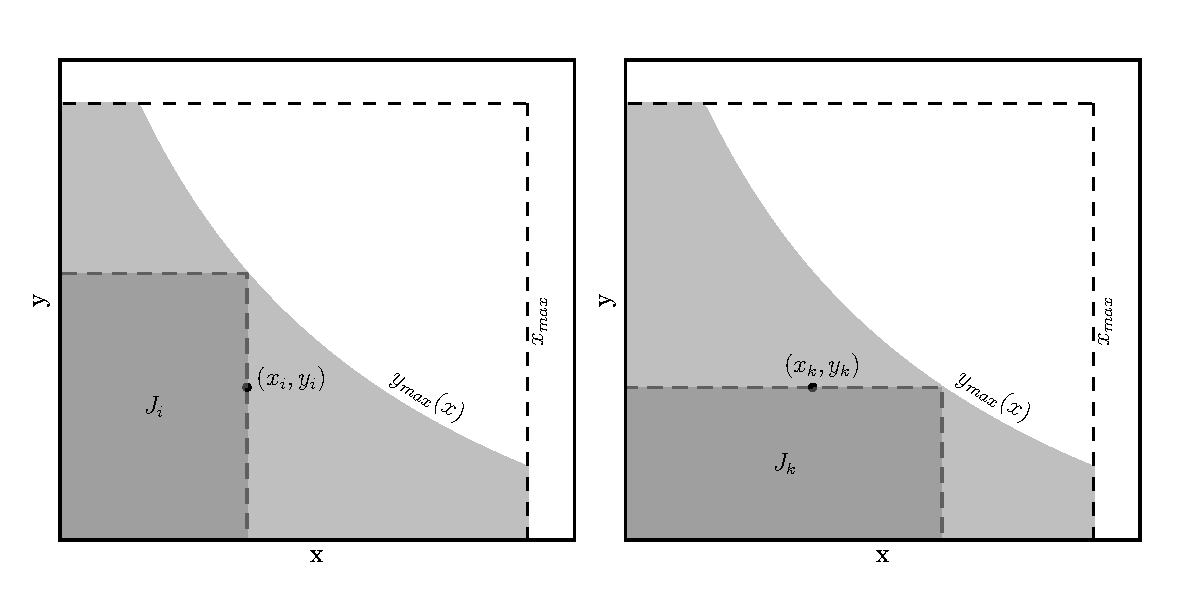
\includegraphics{figures/fig_lyndenbell_setup-1.pdf}}

\vfill
\end{slide}
 



%------------------------------------------------------------------------------
\begin{slide}
\begin{center}
\bfseries
{\large {\color{red} C$^-$ method}}
\end{center}
\vskip 0.2in
\hrule

Assuming that $\tau<1$, it is straightforward to show using relatively simple probability integral 
analysis (e.g., see Appendix in Fan et al. 2001), as well as the original Lynden-Bell's paper,
how to determine cumulative distribution functions.
The cumulative distributions are defined as 
\eq{
             \Phi(x) = \int_{-\infty}^{x} \Psi(x') dx',
}
and 
\eq{
              \Sigma(y) = \int_{-\infty}^y \rho(y') dy'.
}
Then, 
\eq{
              \Phi(x_i) = \Phi(x_1) \, \Pi_{k=2}^i (1 + 1/N_k)
}
where it is assumed that $x_i$ are sorted ($x_1 \le x_k \le x_N$).

\vskip -0.7in
\phantom{x}
%\scalebox{0.9}{\hskip 1.4in 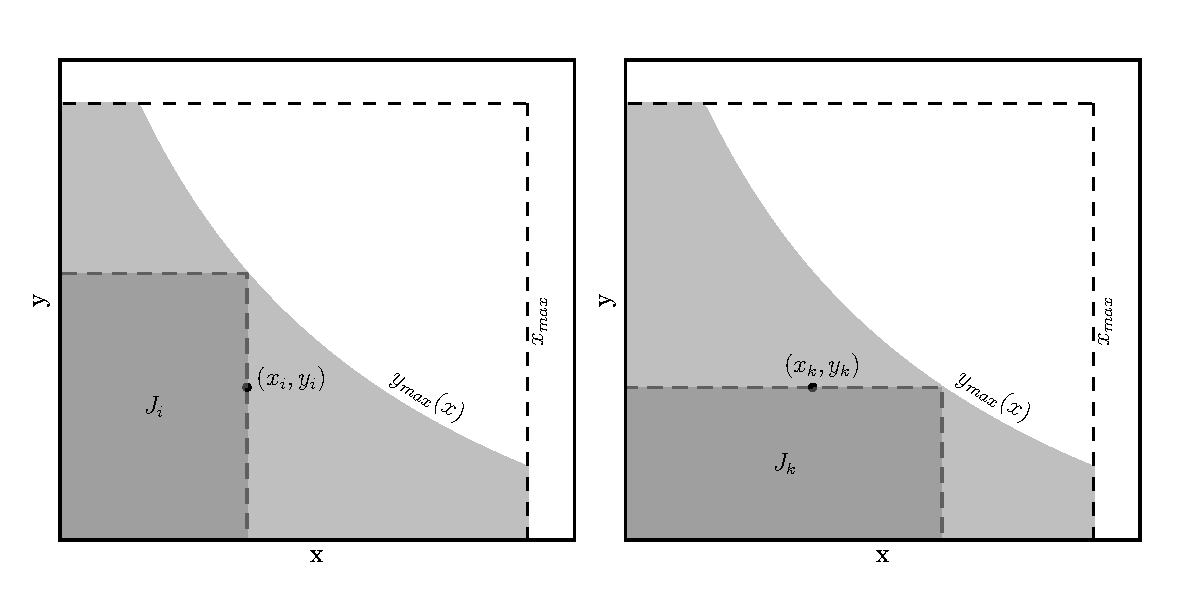
\includegraphics{figures/fig_lyndenbell_setup-1.pdf}}

\vfill
\end{slide}
 

%------------------------------------------------------------------------------
\begin{slide}
\begin{center}
\bfseries
{\large {\color{red} C$^-$ method}}
\end{center}
\vskip 0.2in
\hrule


Analogously, if $M_k$ is the
number of objects in a set defined by $J_k = \{ j:y_j < y_k, y_{max}(x_j) > y_k\}$
(see the right panel of figure below), then
\eq{
              \Sigma(y_j) = \Sigma(y_1) \, \Pi_{k=2}^j (1 + 1/M_k). 
}

\vskip -0.7in
\phantom{x}
\scalebox{0.9}{\hskip 1.4in 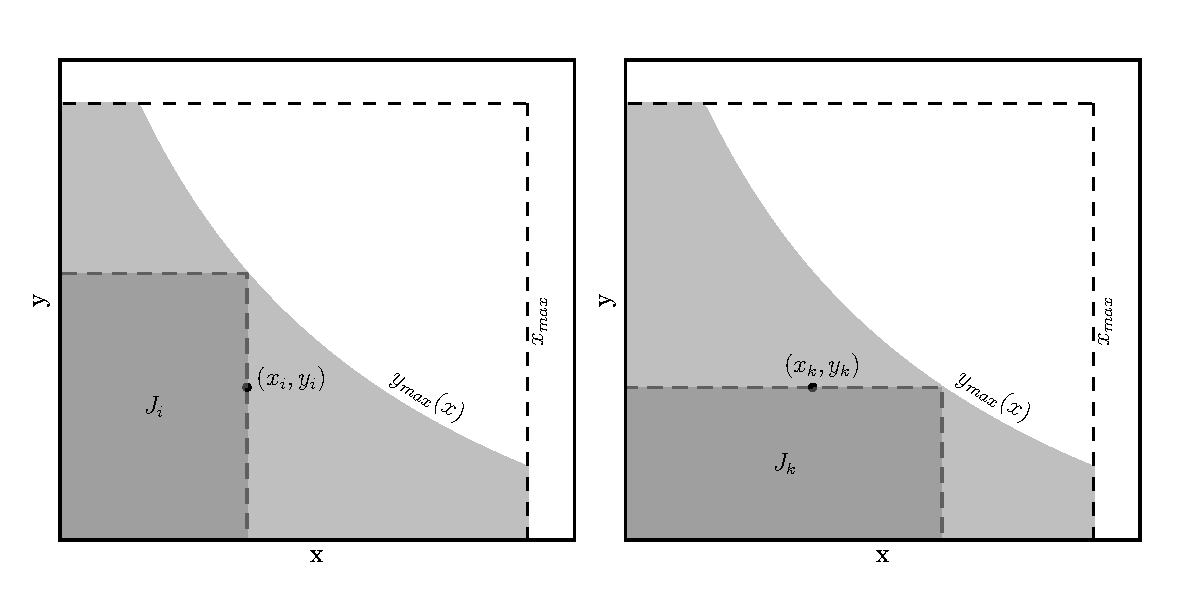
\includegraphics{figures/fig_lyndenbell_setup-1.pdf}}


\vfill
\end{slide}
 


%------------------------------------------------------------------------------
\begin{slide}
\begin{center}
\bfseries
{\large {\color{red} astroML implementation of the C$^-$ method}}
\end{center}
\vskip 0.2in
\hrule

\begin{itemize}
\item 
Note that both $\Phi(x_j)$ and $\Sigma(y_j)$ are defined on non-uniform grids with $N$ values,
corresponding to the $N$ measured values. 
\item 
Essentially, the $C^{-}$ method assumes a piece-wise
constant model for $\Phi(x)$ and $\Sigma(y)$ between data points (equivalently, differential distributions
are modeled as Dirac's $\delta$ functions at the position of each data point). 
\item 
As shown by Petrosian (1992), $\Phi(x)$ and $\Sigma(y)$ represent an optimal data summary. 
\item
The differential distributions $\Psi(x)$ and $\rho(y)$ can be obtained by differentiating cumulative 
distributions in the relevant axis; an approximate normalization can be obtained by requiring that 
the total predicted number of objects is equal to their observed number. 
\end{itemize}

\vskip -0.7in
\phantom{x}
%\scalebox{0.9}{\hskip 1.4in 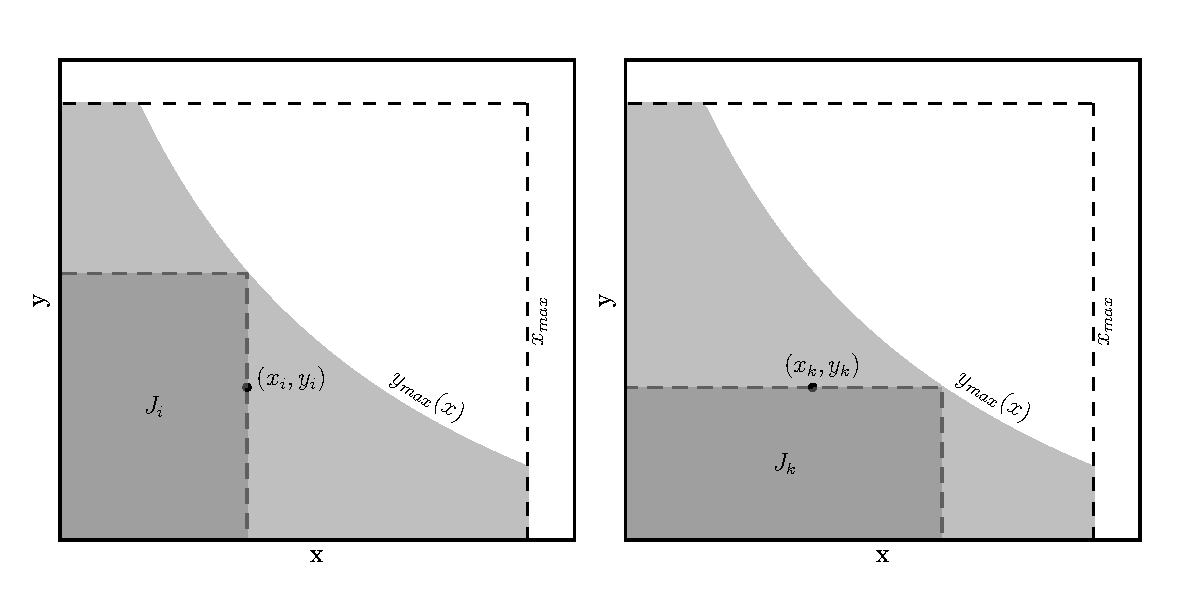
\includegraphics{figures/fig_lyndenbell_setup-1.pdf}}

\vfill
\end{slide}
 


%------------------------------------------------------------------------------
\begin{slide}

\begin{itemize}
\item {\bf astroML Book Figure 4.9:} 
The right panel shows a realization of truncated separable two-dimensional 
Gaussian distribution (with the truncation given by the solid line).
The lines in the left panel show the true one-dimensional distributions of $x$ 
and $y$, and the points are computed from the truncated data set using the $C^-$ method
(with error bars from 20 bootstrap resamples). 
\end{itemize}

\begin{verbatim}
http://astroml.github.com/
book_figures/chapter4/fig_lyndenbell_toy.html
\end{verbatim} 
\vskip -0.7in
\phantom{x}
\scalebox{0.9}{\hskip 0.4in 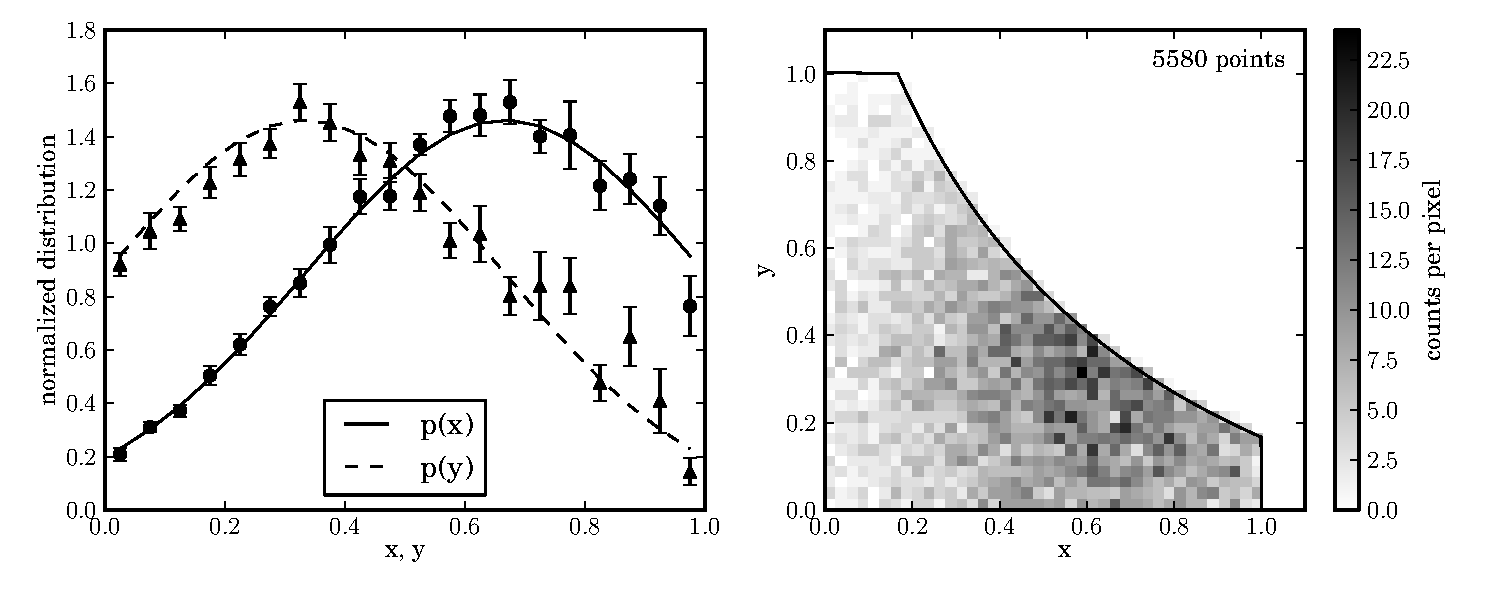
\includegraphics{figures/fig_lyndenbell_toy-1.pdf}}

\vfill
\end{slide}
 

%------------------------------------------------------------------------------
% TWO-SIDED PAGE 
\begin{slide}

\hbox to \hsize{
\begin{minipage}[t]{11cm}
\begin{center}
\vskip 0.4in
\scalebox{0.7}{\hskip -1.4in 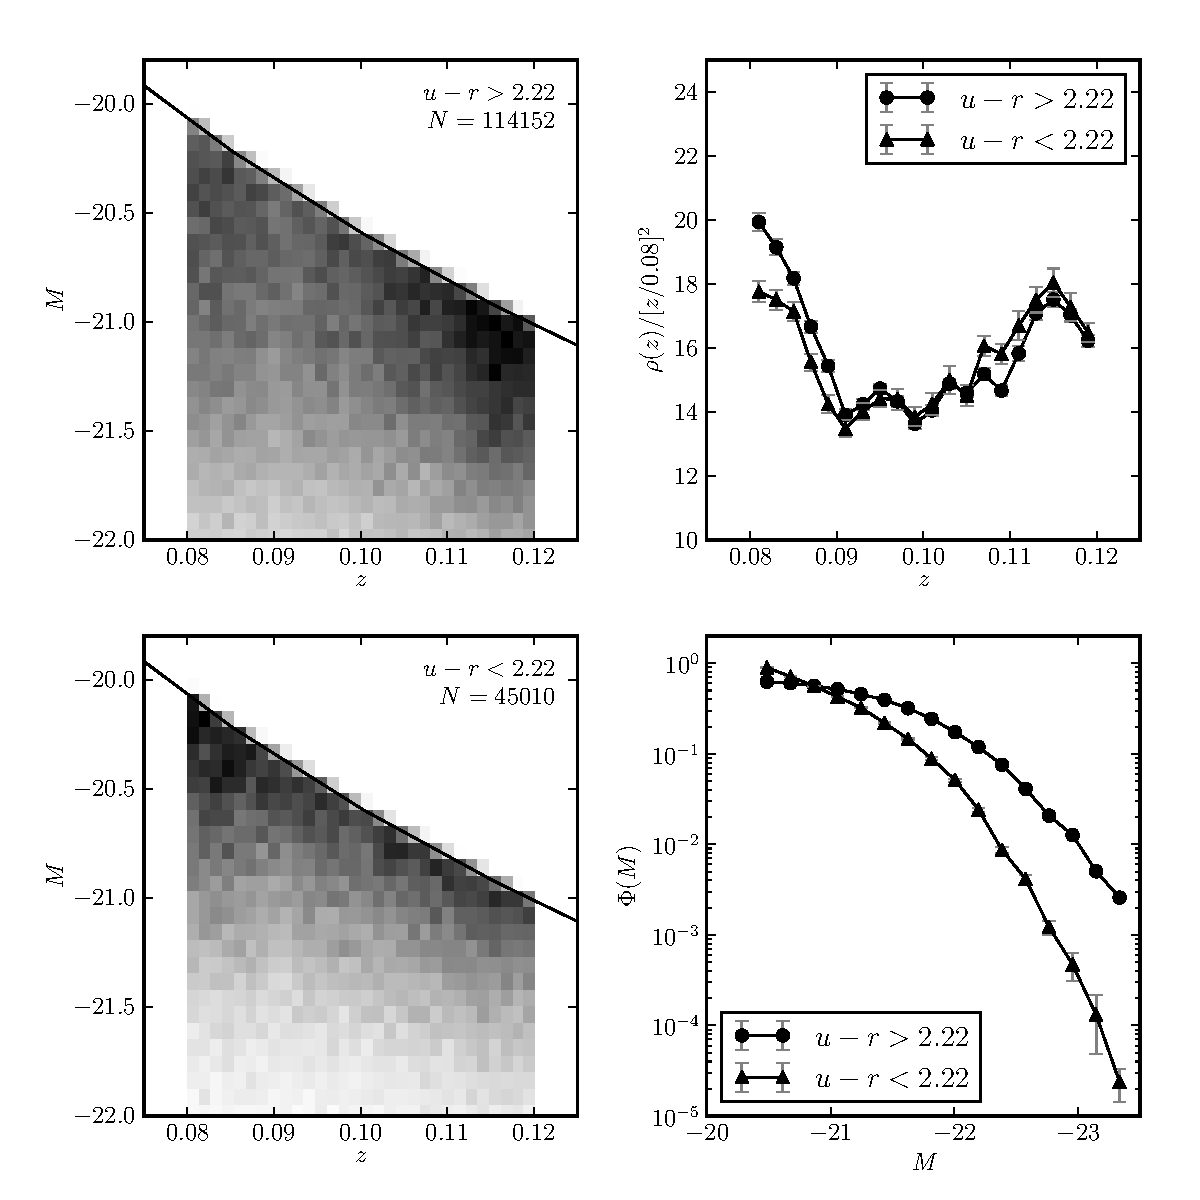
\includegraphics{figures/fig_lyndenbell_gals-1.pdf}}
\end{center}
\vskip 0.3in
\begin{verbatim}
http://astroml.github.com/
book_figures/chapter4/fig_lyndenbell_gals.html
\end{verbatim} 
\end{minipage}

\begin{minipage}[t]{13cm}

\begin{itemize}
\item {\bf astroML Book Figure 4.10:}
The luminosity function for two 
    $u-r$ color-selected subsamples of SDSS galaxies from the spectroscopic sample, with 
    redshift in the range $0.08 < z < 0.12$ and flux limited to $r < 17.7$.  
\item The left
    panels show the distribution of sources as a function of redshift and
    absolute magnitude.  The distribution $p(z, M) = \rho(z)\Phi(m)$ is
    obtained using Lynden-Bell's method, with errors determined by
    20 bootstrap resamples, and  shown in the right panels.
\end{itemize}  
\end{minipage}}
\vfill 
\end{slide}

%------------------------------------------------------------------------------
\begin{slide}
\begin{center}
\bfseries
{\large {\color{red} Test of L-z Correlation. II}}
\end{center}
\vskip 0.2in
\hrule

\begin{itemize}
\item In reality, the selection function is typically complex:
      $s(L,z|SED, ...)$ (no sharp faint limit!)
\item First define a generalized comparable set (Fan et al. 2001;
      AJ 121, 54)
      $J_i = \{ j:L_j > L_i\}$; this is a luminosity limited data 
      subset for object $i$
\item Then generalize $N_i$ to
\begin{equation}
        T_i = \sum_{j=1}^{N_i} {s(L_i, z_j|SED_j) \over s(L_j, z_j|SED_j)},
\end{equation}
and redefine the rank accordingly
\begin{equation}
        R_i = \sum_{j=1}^{N_i} {s(L_i, z_j|SED_j) \over s(L_j, z_j|SED_j)},
\end{equation}
for $z_j < z_i$. It follows that $E(R_i) = T_i/2$ and $V(R_i) = T_i^2/12$. 

\end{itemize}

\vfill
\end{slide}
 


%------------------------------------------------------------------------------
\begin{slide}
\begin{center}
\bfseries
{\large {\color{red} LF normalization}}
\end{center}
\vskip 0.2in
\hrule

\begin{itemize}
\item The C$^-$ method does not know (or need) details about our sample; in particular, 
     it cannot give us the overall LF normalization! 
\item We will use HW\#2 problem to discuss normalization in more detail; we can talk 
about three levels of normalization in this case:
\begin{enumerate} 
\item {\color{blue} The sample normalization:} if we didn't have the selection effects, how many 
  objects would our sample contain? 
\item {\color{blue} Normalization to the full sky:} we need to know the sky coverage for our 
   sample (and have arguments why we can extrapolate to the whole sky). 
\item {\color{blue} Extrapolation}  from the volume probed by the sample  {\color{blue} to some other position;} 
   here, we want to know LF at $Z=0$. 
\end{enumerate} 
\end{itemize}

\vfill
\end{slide}
 
%------------------------------------------------------------------------------
\begin{slide}
\begin{center}
\bfseries
{\large {\color{red} LF normalization: the sample normalization}}
\end{center}
\vskip 0.2in
\hrule
{\color{blue} If we didn't have the selection effects, how many 
  objects would our sample contain?} 
\begin{itemize}
\item  To recap, the cumulative luminosity (absolute magnitude) function is 
$\Phi_c(M_j)$ and the cumulative distance distribution is $n_c(D_j)$ where
$j=1...N$.
\item Both $\Phi_c(M_j)$ and $n_c(D_j)$ are  {\color{blue} direct outputs} from the C$^-$ method;
{\color{blue} let us renormalize them} as $\Phi_c(M_N)=1$ and  $n_c(D_N)=1$,
where it is assumed that $M_j$ and $D_j$ arrays are sorted so that $M_N$ and 
$D_N$ are their maxima (btw, C$^-$ would return $\Phi_c(M_N)=N$ and  $n_c(D_N)=N$). 
\item The number of points, $n$,  brighter than some arbitrary $M^\ast$ and closer than $D^\ast$ is then
\begin{equation}
          n(M<M^\ast \,\, {\rm and} \,\,  D<D^\ast)= C \, \Phi_c(M^\ast) \, n_c(D^\ast).
\end{equation}
where we (still) don't know $C$ (n.b. $C$ is dimensionless). 
\end{itemize}

\vfill
\end{slide}
 

%------------------------------------------------------------------------------
\begin{slide}
\begin{center}
\bfseries
{\large {\color{red} LF normalization: the sample normalization}}
\end{center}
%\vskip 0.2in
\hrule
\begin{itemize}
\item Now, if make sure that $M^\ast$ and $D^\ast$ are {\color{blue} within our selection volume} 
(the implied apparent mag must be above our cutoff)
and thus  {\color{blue} unaffected by selection effects,} then we get $C$ from
\begin{equation}
          N^o(M<M^o \,\, {\rm and} \,\,  D<D^o)= C \, \Phi_c(M^o) \, n_c(D^o),
\end{equation}
which is almost the same expression as on the previous page, except that here 
$n(M<M^\ast \,\, {\rm and} \,\,  D<D^\ast)$ is replaced by $N^o(M<M^o \,\, {\rm and} \,\,  D<D^o)$:
{\color{blue} the actual number of objects in our sample that satisfy this condition.}
\item This is not mathematically optimal solution for $C$ because  $N^o$ is a random variable, 
but with modern large samples this is nit-picking; the optimal procedure would integrate over the
full sample, but nevertheless would still need to adopt an interpolation procedure for 
$\Phi_c(M)$ and $n_c(D)$...
\item  {\color{blue} Given the real sample size, $N$, that is affected by selection effects,  the ``corrected'' sample
size is $C$!}
\end{itemize}
\vfill
\end{slide}
 

%------------------------------------------------------------------------------
\begin{slide}
\begin{center}
\bfseries
{\large {\color{red} LF normalization: the sample normalization}}
\end{center}
\vskip 0.2in
\hrule
\begin{itemize} 
\item The number of points per unit two-dimensional area, $dA = dM \, dD$, is then
\begin{equation}
  {d^2 N \over dM dD } = C \, \left( {d \Phi_c(M) \over dM } \right) \, \left( {d n_c(D) \over d D} \right),
\end{equation}
where we now know $C$ and can easily take (numerical) derivatives  ${d \Phi_c(M) / dM }$ and
${d n_c(D) / d D}$ (where $\Phi_c(M)$ and $n_c(D)$ came from $C^-$ and are normalized to 1). 
\item The quantities in parenthesis are differential distribution functions.
\item  When normalizing to the full sky (step \#2), we need to know the fraction of sky, $f_{sky}$,
covered by our sample; if justified, we need to multiply $C$ by $1/f_{sky}$: $C_{sky} = C / f_{sky}$. 
\end{itemize}

\vfill
\end{slide}
 


 
%------------------------------------------------------------------------------
\begin{slide}
\begin{center}
\bfseries
{\large {\color{red} LF normalization: extrapolation}}
\end{center}
\vskip 0.2in
\hrule
{\color{blue} How do we go from $d^2 N / (dM dD)$ to volume density? } 
\begin{equation}
  \Phi(M,D) \equiv  {d^2 N \over dM dV } =    {d^2 N \over dM dD }  \, {dD \over dV},
\end{equation}
where $dV = 4\pi D^2 dD$. We have two cases of interest: 
\begin{itemize}
\item {\bf Case 1:} We seek the volume density vs. D, $\rho(D)$, and we don't care about $M$ distribution:
\begin{equation}
   \rho(D) = \int \Phi(M,D) dM = {C_{sky} \over 4\pi D^2} \, \left( {d n_c(D) \over d D} \right),
\end{equation}
where we used the fact that $\int_{-\infty}^\infty  \left( {d \Phi_c(M) \over dM } \right)   dM = \Phi_c(M_N)=1$. 
\item Unit for $\rho(D)$ is the number of objects per (distance unit)$^3$ (remember that 
$n_c(D)$ was dimensionless and normalized to unity at $D=D_N$; the unit comes from 
taking derivative with respect to $D$, $d n_c(D) /d D$).  
\end{itemize}

\vfill
\end{slide}
 
%------------------------------------------------------------------------------
\begin{slide}
\begin{center}
\bfseries
{\large {\color{red} LF normalization: extrapolation}}
\end{center}
\vskip 0.2in
\hrule
\begin{itemize}
\item Given $\rho(D)$, we can fit some function to it and {\bf extrapolate} to get $\rho(D=D_0)$
(and thus the ratio $\rho(D)/\rho(D=D_0)$ for any $D_0$, including $\rho(D_0)/\rho(D_N)$). 
\item {\bf Case 2:} We want to know the $M$ distribution at some $D=D_0$, call it  $\psi(M | D=D_0) $ 
(e.g. $D_0=0$ corresponding to solar neighborhood, as discussed in this HW). First, at $D=D_N$
(recall  $n_c(D_N)=1$)
\begin{equation}
   \psi(M | D=D_N) = \int \Phi(M,D) dD = C_{sky} \, \left( {d \Phi_c(M) \over dM } \right). 
\end{equation}
\item Then, extrapolating to $D_0$ (unit for $\psi$ is the number of objects per mag; this
is what we compare to the ``true'' LF)
\begin{equation}
   \psi(M | D=D_0) =  \psi(M | D=D_N) \, {\rho(D_0)  \over \rho(D_N) }.
\end{equation}
\end{itemize}

\vfill
\end{slide}
 

 







%------------------------------------------------------------------------------
\begin{slide}
\begin{center}
\bfseries
{\large {\color{red} Evolving Luminosity Function}}
\end{center}
\vskip 0.2in
\hrule

\begin{itemize}
\item The C$^-$ method is simple and optimal, but it is valid only 
      for uncorrelated variables (separable luminosity function). 
      What do we do when the $\tau$ test suggests correlated 
      variables? 
\item Recent work by Kelly, Fan and Vestergaard (2008, ApJ 682, 874)
      describes a powerful and completely general Bayesian approach
      (see their Appendix A for a nice introduction to Bayesian methodology). 
      While too complex for homework, this is a fantastic method -- if you ever
      come again across the problem of estimating a general multi-dimensional
      distribution that is sampled with non-negligible and possibly 
      complex selection function, remember it!
\end{itemize}

\vfill
\end{slide}
 

%------------------------------------------------------------------------------
\begin{slide}
\begin{center}
\bfseries
{\large {\color{red} Stellar Mass Function}}
\end{center}
\vskip 0.2in
\hrule

\begin{itemize}
\item Analogously to luminosity function, the mass function is the distribution of mass of stars,
galaxies, etc. 
\item The term {\it Stellar mass function} can refer to the distribution of galaxies with respect
to their stellar mass (mass of all their stars), or to the distribution of mass of stars in the Milky Way! 
\item The distribution of mass of stars in the Milky Way is often parametrized by a power law, $dN/dM \propto M^{-\alpha}$,
with $\alpha=2.35$ (called Salpeter function in this context; FYI: power law is called the Pareto distribution in statistics...)
\item Kroupa, Tout \& Gilmore (1993, MNRAS 262, 545) proposed a three-part power law
\end{itemize}

\vfill
\end{slide}
 


%------------------------------------------------------------------------------
% TWO-SIDED PAGE 
\begin{slide}

\hbox to \hsize{
\begin{minipage}[t]{12cm}
\begin{center}
\vskip 0.0in
\scalebox{0.9}{\hskip -1.4in 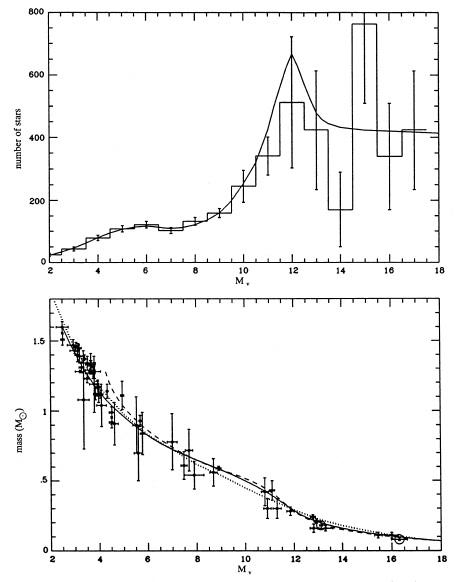
\includegraphics{figures/massfunction1.jpg}}
\end{center}
\end{minipage}

\begin{minipage}[t]{12cm}
\begin{center}
\vskip -1in
{\large \color{red} Mass Function of Disk stars}
\end{center}

\begin{itemize}
\item Determination of a three-part power law mass function by Kroupa, Tout \& Gilmore (1993)
\item Top: the measured number of stars per $M_V$ bin
\item Bottom: the mass-luminosity relation adopted in deriving the mass function 
\end{itemize}  

\end{minipage}}
\vfill 
\end{slide}
%------------------------------------------------------------------------------

%------------------------------------------------------------------------------
% TWO-SIDED PAGE 
\begin{slide}

\hbox to \hsize{
\begin{minipage}[t]{12cm}
\begin{center}
\vskip 0.0in
\scalebox{0.9}{\hskip -1.2in 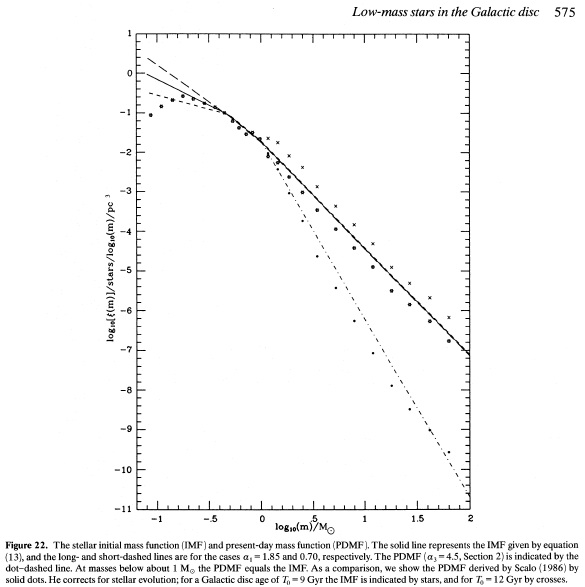
\includegraphics{figures/massfunction2.jpg}}
\end{center}
\end{minipage}

\begin{minipage}[t]{12cm}
\begin{center}
\vskip 0.1in
{\large \color{red} \phantom{x} Mass Function of Disk stars}
\end{center}

\begin{itemize}
\item Determination of a three-part power law mass function by Kroupa, Tout \& Gilmore (1993)
\item Present-day mass function (PDMF): dot-dashed line
\item Initial mass function (IMF): solid line
\item Note that the PDMF and IMF are equal below about 1 solar mass.
\end{itemize}  

\end{minipage}}
\vfill 
\end{slide}
%------------------------------------------------------------------------------


%------------------------------------------------------------------------------
% TWO-SIDED PAGE 
\begin{slide}

\hbox to \hsize{
\begin{minipage}[t]{12cm}
\begin{center}
\vskip -0.7in
\scalebox{0.6}{\hskip -1.2in 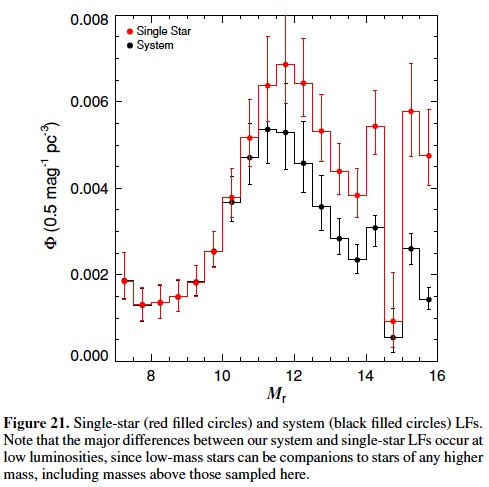
\includegraphics{figures/massfunction3a.jpg}}
\vskip -0.05in
\scalebox{0.65}{\hskip -1.2in 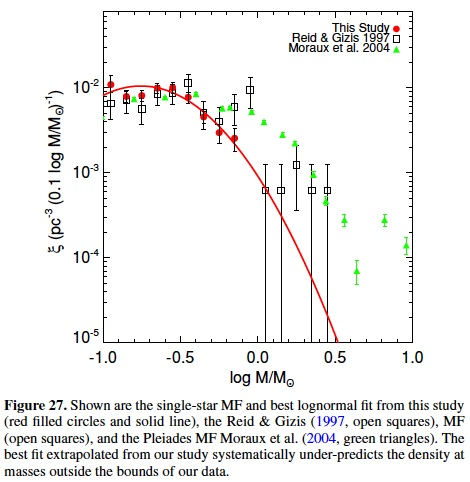
\includegraphics{figures/massfunction3b.jpg}}
\end{center}
\end{minipage}

\begin{minipage}[t]{12cm}
\begin{center}
\vskip 0.1in
{\large \color{red} \phantom{x} Luminosity and Mass Function of Low-mass stars}
\end{center}

\begin{itemize}
\item Bochanski et al. (2010, AJ 139, 2679)
\item Based on SDSS data for 15 million low-mass stars! 
\item The mass range: 0.1--0.8 solar masses (corresponding to $7 < M_r < 16$)
\item The turn-over and a local maximum well detected! 
\item Data well described by a log-normal distribution (over the probed mass range). 
\end{itemize}  

\end{minipage}}
\vfill 
\end{slide}
%------------------------------------------------------------------------------


%------------------------------------------------------------------------------
% TWO-SIDED PAGE 
\begin{slide}

\hbox to \hsize{
\begin{minipage}[t]{12cm}
\begin{center}
\vskip 0.4in
\scalebox{0.6}{\hskip -1.4in 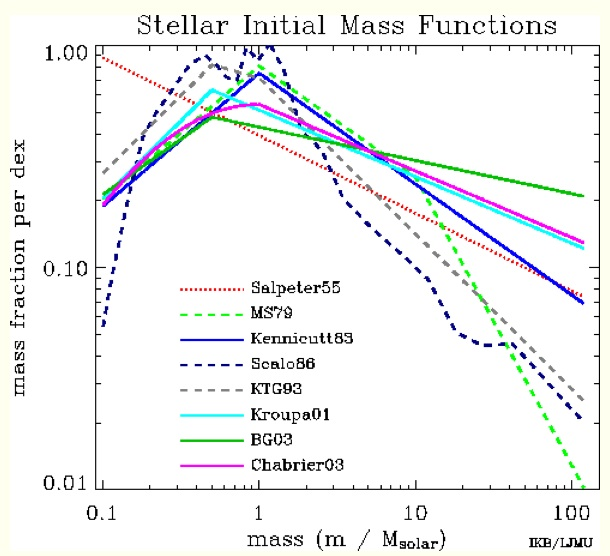
\includegraphics{figures/IMFcomparison.jpg}}
\vskip 0.3in
{
From Ivan Baldry: 
\begin{verbatim}
http://www.astro.ljmu.ac.uk/~ikb/research/imf-use-in-cosmology.html
\end{verbatim}
}
\end{center}
\end{minipage}

\begin{minipage}[t]{12cm}
\begin{center}
\vskip 0.0in
{\large \color{red} Initial Mass Function}
\end{center}

\begin{itemize}
\item {\colour{blue} The stellar initial mass function (IMF)} is used for computing stellar masses and 
colors of galaxies in cosmology.
\item There is substantial variation between different estimates (left). 
\item Kroupa (2001) claimed a variable IMF (MNRAS 322, 231).
\end{itemize}  

\end{minipage}}
\vfill 
\end{slide}
%------------------------------------------------------------------------------



%------------------------------------------------------------------------------
% TWO-SIDED PAGE 
\begin{slide}

\hbox to \hsize{
\begin{minipage}[t]{12cm}
\begin{center}
\vskip -0.1in
\scalebox{1.0}{\hskip -0.8in 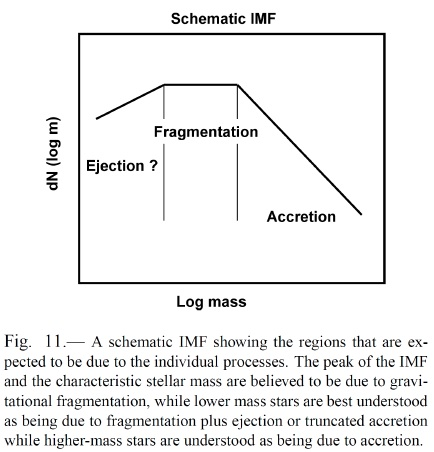
\includegraphics{figures/massfunction4.jpg}}
\vskip 0.3in
{
From W. Chen
}
\end{center}
\end{minipage}

\begin{minipage}[t]{12cm}
\begin{center}
\vskip 0.0in
{\large \color{red} Initial Mass Function}
\end{center}

\begin{itemize}
\item An approximate understanding of the origin of different slopes.
\item A hard problem to solve! (e.g. turbulence, magnetic fields...) 
\end{itemize}  

\end{minipage}}
\vfill 
\end{slide}
%------------------------------------------------------------------------------




%%%%%%%%%%%%%%%%
\end{document}



%------------------------------------------------------------------------------
\begin{slide}
\begin{center}
\bfseries
{\large {\color{red} Stellar Function}}
\end{center}
\vskip 0.2in
\hrule

\begin{itemize}
\item 
\end{itemize}

\vfill
\end{slide}
 



